%\documentclass{beamer}
\documentclass[handout]{beamer}

\usepackage{amsmath}
\usepackage{beamerthemesplit}
\usepackage{fancybox}
\usepackage{hyperref}
\usepackage{color}
\usepackage{listings}


\makeatletter
\newcommand\code{\bgroup\@makeother\_\@makeother\~\@makeother\$\@codex}
\def\@codex#1{{\normalfont\ttfamily\hyphenchar\font=-1 #1}\egroup}
\makeatother

\newcommand{\bX}{\boldsymbol{X}}
\newcommand{\bx}{\boldsymbol{x}}
\newcommand{\by}{\boldsymbol{y}}
\newcommand{\bbeta}{\boldsymbol{\beta}}
\newcommand{\bepsilon}{\boldsymbol{\epsilon}}
\newcommand{\bs}[1]{\boldsymbol{#1}}


\definecolor{gray}{rgb}{.6,.6,.6}
\definecolor{orange}{rgb}{1,0.5,0}
\definecolor{grayish}{rgb}{.775, .775, .775}
\definecolor{dkgray}{rgb}{.375, .375, .375}
\definecolor{dkgreen}{rgb}{0,0.6,0}
\definecolor{mauve}{rgb}{0.58,0,0.82}
\definecolor{dkblue}{rgb}{0, 0, .5}
\definecolor{purple}{rgb}{0.7, 0, 0.5}

\definecolor{g11}{rgb}{0, 0, 1}
\definecolor{g12}{rgb}{0, .4, 1}
\definecolor{g13}{rgb}{0, .8, 1}

\definecolor{g21}{rgb}{0, .5, .3}
\definecolor{g22}{rgb}{.4, .5, .3}
\definecolor{g23}{rgb}{.8, .5, .3}

\lstset{ %
  language=R,     
  numbers=left,
  stepnumber=1,       
  numbersep=6pt,      
  showspaces=false,      
  showstringspaces=false,  
  showtabs=false,    
  frame=single,      
  rulecolor=\color{black},   
  tabsize=4,     
  captionpos=t,     
  breaklines=true,     
  breakatwhitespace=true,   
  title=\lstname,              
  basicstyle=\ttfamily\color{black}\scriptsize, 
  backgroundcolor=\color{grayish},  
  numberstyle=\tiny\color{black},  
  keywordstyle=\color{blue}, 
  commentstyle=\color{dkgreen}, 
  stringstyle=\color{mauve}, 
  xleftmargin=.1in,
  xrightmargin=.1in,
  aboveskip=0cm,
  belowskip=.2cm
  %   escapeinside={\%*}{*)},    
%   morekeywords={*,...}    
}

\setbeamertemplate{navigation symbols}{} 

\hypersetup{
    linkcolor=,
    colorlinks=true,
    urlcolor=blue
}

\usetheme{Frankfurt}
% \usecolortheme{whale}
% \usetheme{Antibes}
% \setbeamertemplate{mini frames}{}


\newcommand{\fctn}[1]{\textcolor{green!50!blue}{#1}}
\newcommand{\rfor}[1]{\textcolor{yellow!50!red}{#1}}
\newcommand{\rcom}[1]{\textcolor{blue}{#1}}

\newcommand{\pkg}[1]{\textbf{#1}}

\newcommand{\startr}{\begin{minipage}{.04\textwidth}\ \ \end{minipage} \begin{minipage}{.91\textwidth}}

%
\newcommand{\shownum}{\title[\mytitlea]}{}
\newcommand{\hidenum}{\title[\mytitleb]{}}
% \expandafter\def\expandafter\insertshorttitle\expandafter{\insertshorttitle\hfill\insertframenumber\,/\,\inserttotalframenumber}
 

\newcounter{excount}
\setcounter{excount}{0}
\newcommand{\countex}{\addtocounter{excount}{1}\arabic{excount}}
\newcommand{\showex}{\arabic{excount}}






\useoutertheme{miniframes}
\makeatletter
  \beamer@compressfalse
\makeatother

\title{From 1 core to Thousands: R to pbdR}
\author[http://r-pbd.org \hspace{2cm}  pbdR Core Team]{%
  George Ostrouchov$^{1,2}$ and Drew Schmidt$^2$
%  and Wei-Chen Chen$^1$,
%  and Pragneshkumar Patel$^2$
\\[1em]
{$^1$Oak Ridge National Laboratory, Oak Ridge, TN} \\
{$^2$University of Tennessee, Knoxville, TN} \\[5em]
OLCF Workshop \\ on  Processing and Analysis of Very Large Data Sets \\
August 8, 2013}
\date{}
\logo{
  \begin{tabular}{r}
    
\includegraphics[height=.34cm]{../common/pics/ornl.jpg} \\
    
\includegraphics[height=.34cm]{../common/pics/utk_logo.png}
  \end{tabular}
}

\newcommand{\mytitlea}{From 1 core to Thousands: R to pbdR \hspace{1cm} \insertframenumber\,/\,\inserttotalframenumber}
\newcommand{\mytitleb}{From 1 core to Thousands: R to pbdR}

%%%%%%%%%%%%%%%%%%%%%%%%%%%%%%%%%%%%%%%%%%%%%%%%%%%%%%%%%%%%%%%%%%%%%%%%%%%%%%%%%
%%%%%%%%%%%%%%%%%%%%%%%%%%%%%%%%%%%%%%%%%%%%%%%%%%%%%%%%%%%%%%%%%%%%%%%%%%%%%%%%%
%%%%%%%%%%%%%%%%%%%%%%%%%%%%%%%%%%%%%%%%%%%%%%%%%%%%%%%%%%%%%%%%%%%%%%%%%%%%%%%%%
\begin{document}

%%%%%%%%%%%%%%%%%%%%%%%%%%%%%%%%%%%%%%%%
%%     Title and ToC
%%%%%%%%%%%%%%%%%%%%%%%%%%%%%%%%%%%%%%%%
% titlepage
\frame{\maketitle}

\setcounter{footnote}{0}

\begin{frame}[noframenumbering]
\frametitle{The \pbdR\ Core Team}
\begin{minipage}{1\textwidth}
  \vspace{-.6cm}
\begin{minipage}{3.6cm}
\ \\[.8cm]
Wei-Chen Chen$^1$ \\
George Ostrouchov$^{2,3}$ \\
Pragneshkumar Patel$^3$ \\
Drew Schmidt$^3$\\[2ex]
\end{minipage}
\begin{minipage}{7cm}
  \ \hfill 
\includegraphics[width=5.5cm]{../common/pics/logos/newpbdr}
\end{minipage}
\end{minipage}
  \begin{minipage}{2.2cm}\tiny
    $^1$FDA\\
    Washington, DC, USA
  \end{minipage}
  \hspace{1ex}
  \begin{minipage}{5cm}\tiny
    $^2$Computer Science and Mathematics Division\\
    Oak Ridge National Laboratory, Oak Ridge TN, USA
  \end{minipage}
  \hspace{1ex}
  \begin{minipage}{4cm}\tiny
    $^3$Joint Institute for Computational Sciences\\
    University of Tennessee, Knoxville TN, USA
  \end{minipage}

\begin{block}{Support}\tiny
  This material is based upon work supported by the National Science
  Foundation Division of Mathematical Sciences under Grant No. 1418195.
  This work used resources of the \textcolor{blue}{National Institute for
  Computational Sciences} at the University of Tennessee, Knoxville,
  which is supported by the Office of Cyberinfrastructure of the
  U.S. National Science Foundation under Award  No. ARRA-NSF-OCI-0906324
  for NICS-RDAV center.
  This work also used resources of the \textcolor{blue}{Oak Ridge
  Leadership Computing Facility} at the Oak Ridge National
  Laboratory, which is supported by the Office of Science of the
  U.S. Department of Energy under Contract No. DE-AC05-00OR22725.\\[.2cm]
\end{block}
\end{frame}

\begin{frame}
  \frametitle{About This Presentation}
  \begin{block}{Downloads}\scriptsize
    You can update the \pbdR presentations and scripts in your virtual
    machine with: \\ \tt
    \$ cd \\
    \$ scp USERNAME@anselm.it4i.cz:/home/adios/slides/pbdr\_overview.pdf slides \\
    \$ scp
    USERNAME@anselm.it4i.cz:/home/adios/slides/pbdr\_tutorial.pdf
    slides \\
    rm -r scripts \\
    \$ scp -r USERNAME@anselm.it4i.cz:/home/adios/pbdR/scripts .
 \end{block}
\end{frame}

% \begin{frame}
% \frametitle{About This Presentation}
%   \begin{block}{Tutorial Evaluations}
%     \begin{center}
%       \url{http://bit.ly/sc13-tut-mf08}
%     \end{center}
%   \end{block}
% \end{frame}


\begin{frame}
\frametitle{About This Presentation}
 \begin{block}{Installation Instructions}
  Installation instructions for setting up a \pbdR environment are available:
  \begin{center}
  \url{http://r-pbd.org/install.html}
  \end{center}
  This includes instructions for installing R, MPI, and \pbdR.
 \end{block}
\end{frame}

% \begin{frame}%[allowframebreaks=0.8]
% \frametitle{About This Presentation}
%  \begin{block}{Conventions}
%   \begin{itemize}
%     \item We use ``{\Huge$ .$}'' as a decimal mark, not ``{\Huge$,$}''.  E.g.,
% 	``one thousand and one half'' is written ``$1,000.5$'', not ``$1.000,5$''.
%     \item We will use special suffixes to denote distributed objects (ones not
% 	stored entirely on a single processor).\\
%     \code{.spmd} denotes a distributed object, while\\
%     \code{.dmat} denotes a distributed object which is of class
% 	\code{ddmatrix}\\
%     No suffix means the object is global (common to all processors)\\[.2cm]
%     Neither of these suffices carries semantic meaning.
%     \end{itemize}
%  \end{block}
% \end{frame}



% \begin{frame}[fragile]
% \frametitle{About This Presentation}
%  \begin{block}{Conventions For Code Presentation}
% We will use two different forms of syntax highlighting.  One for displaying
% results from an interactive R session:
% \begin{lstlisting}[backgroundcolor=\color{white},basicstyle=\ttfamily\color{
% dkgray}\scriptsize,keywordstyle=\color{black},
%   commentstyle=\color{orange},stringstyle=\color{mauve}]
% R> "interactive"
% [1] "interactive"
% \end{lstlisting}
% and one for presenting R scripts
% \begin{lstlisting}
% "not interactive"
% \end{lstlisting}
%  \end{block}
% \end{frame}



\begin{frame}[noframenumbering,shrink]
\frametitle{Contents}
\small
\tableofcontents[hideallsubsections]
\end{frame}

\setcounter{framenumber}{0}
\section{Introduction}
\makesubcontentsslides


%%% Hardware slides
% \subsection{Quick Overview of Parallel Hardware}

\begin{frame}
\begin{block}{Three Basic Flavors of Hardware}
    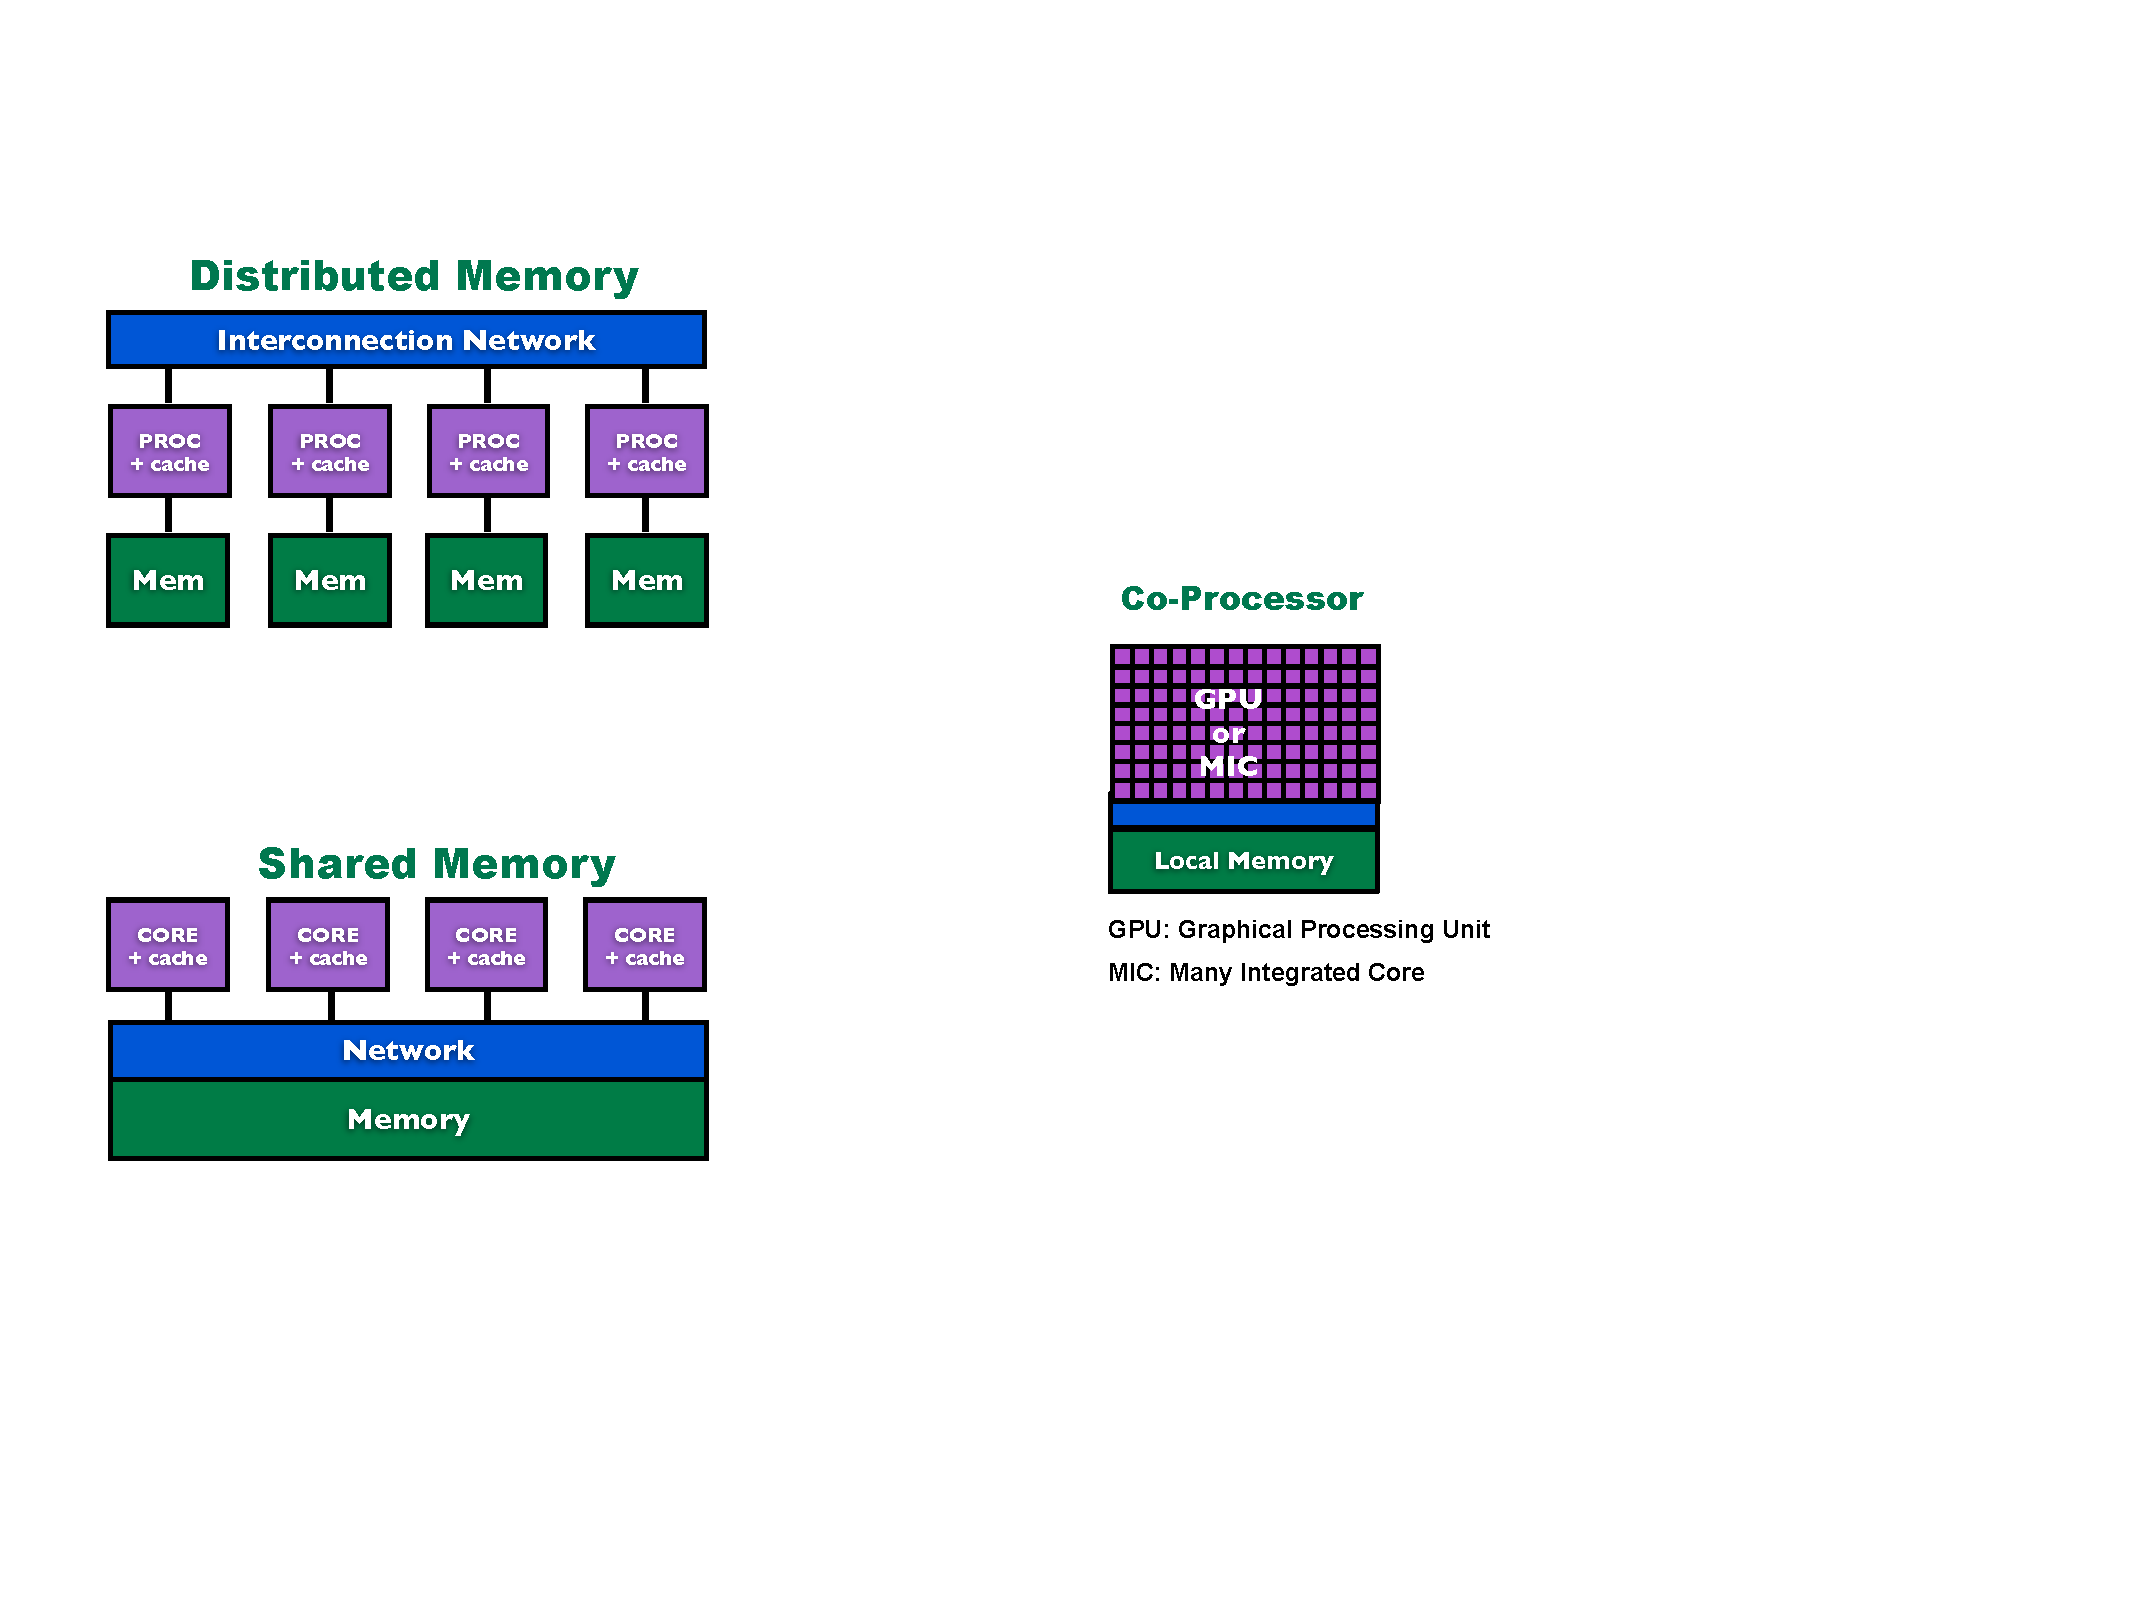
\includegraphics[width=0.95\textwidth]{../common/pics/ParallelHardware1.pdf}
\end{block}
\end{frame}

\begin{frame}
\begin{block}{Your Laptop or Desktop}
    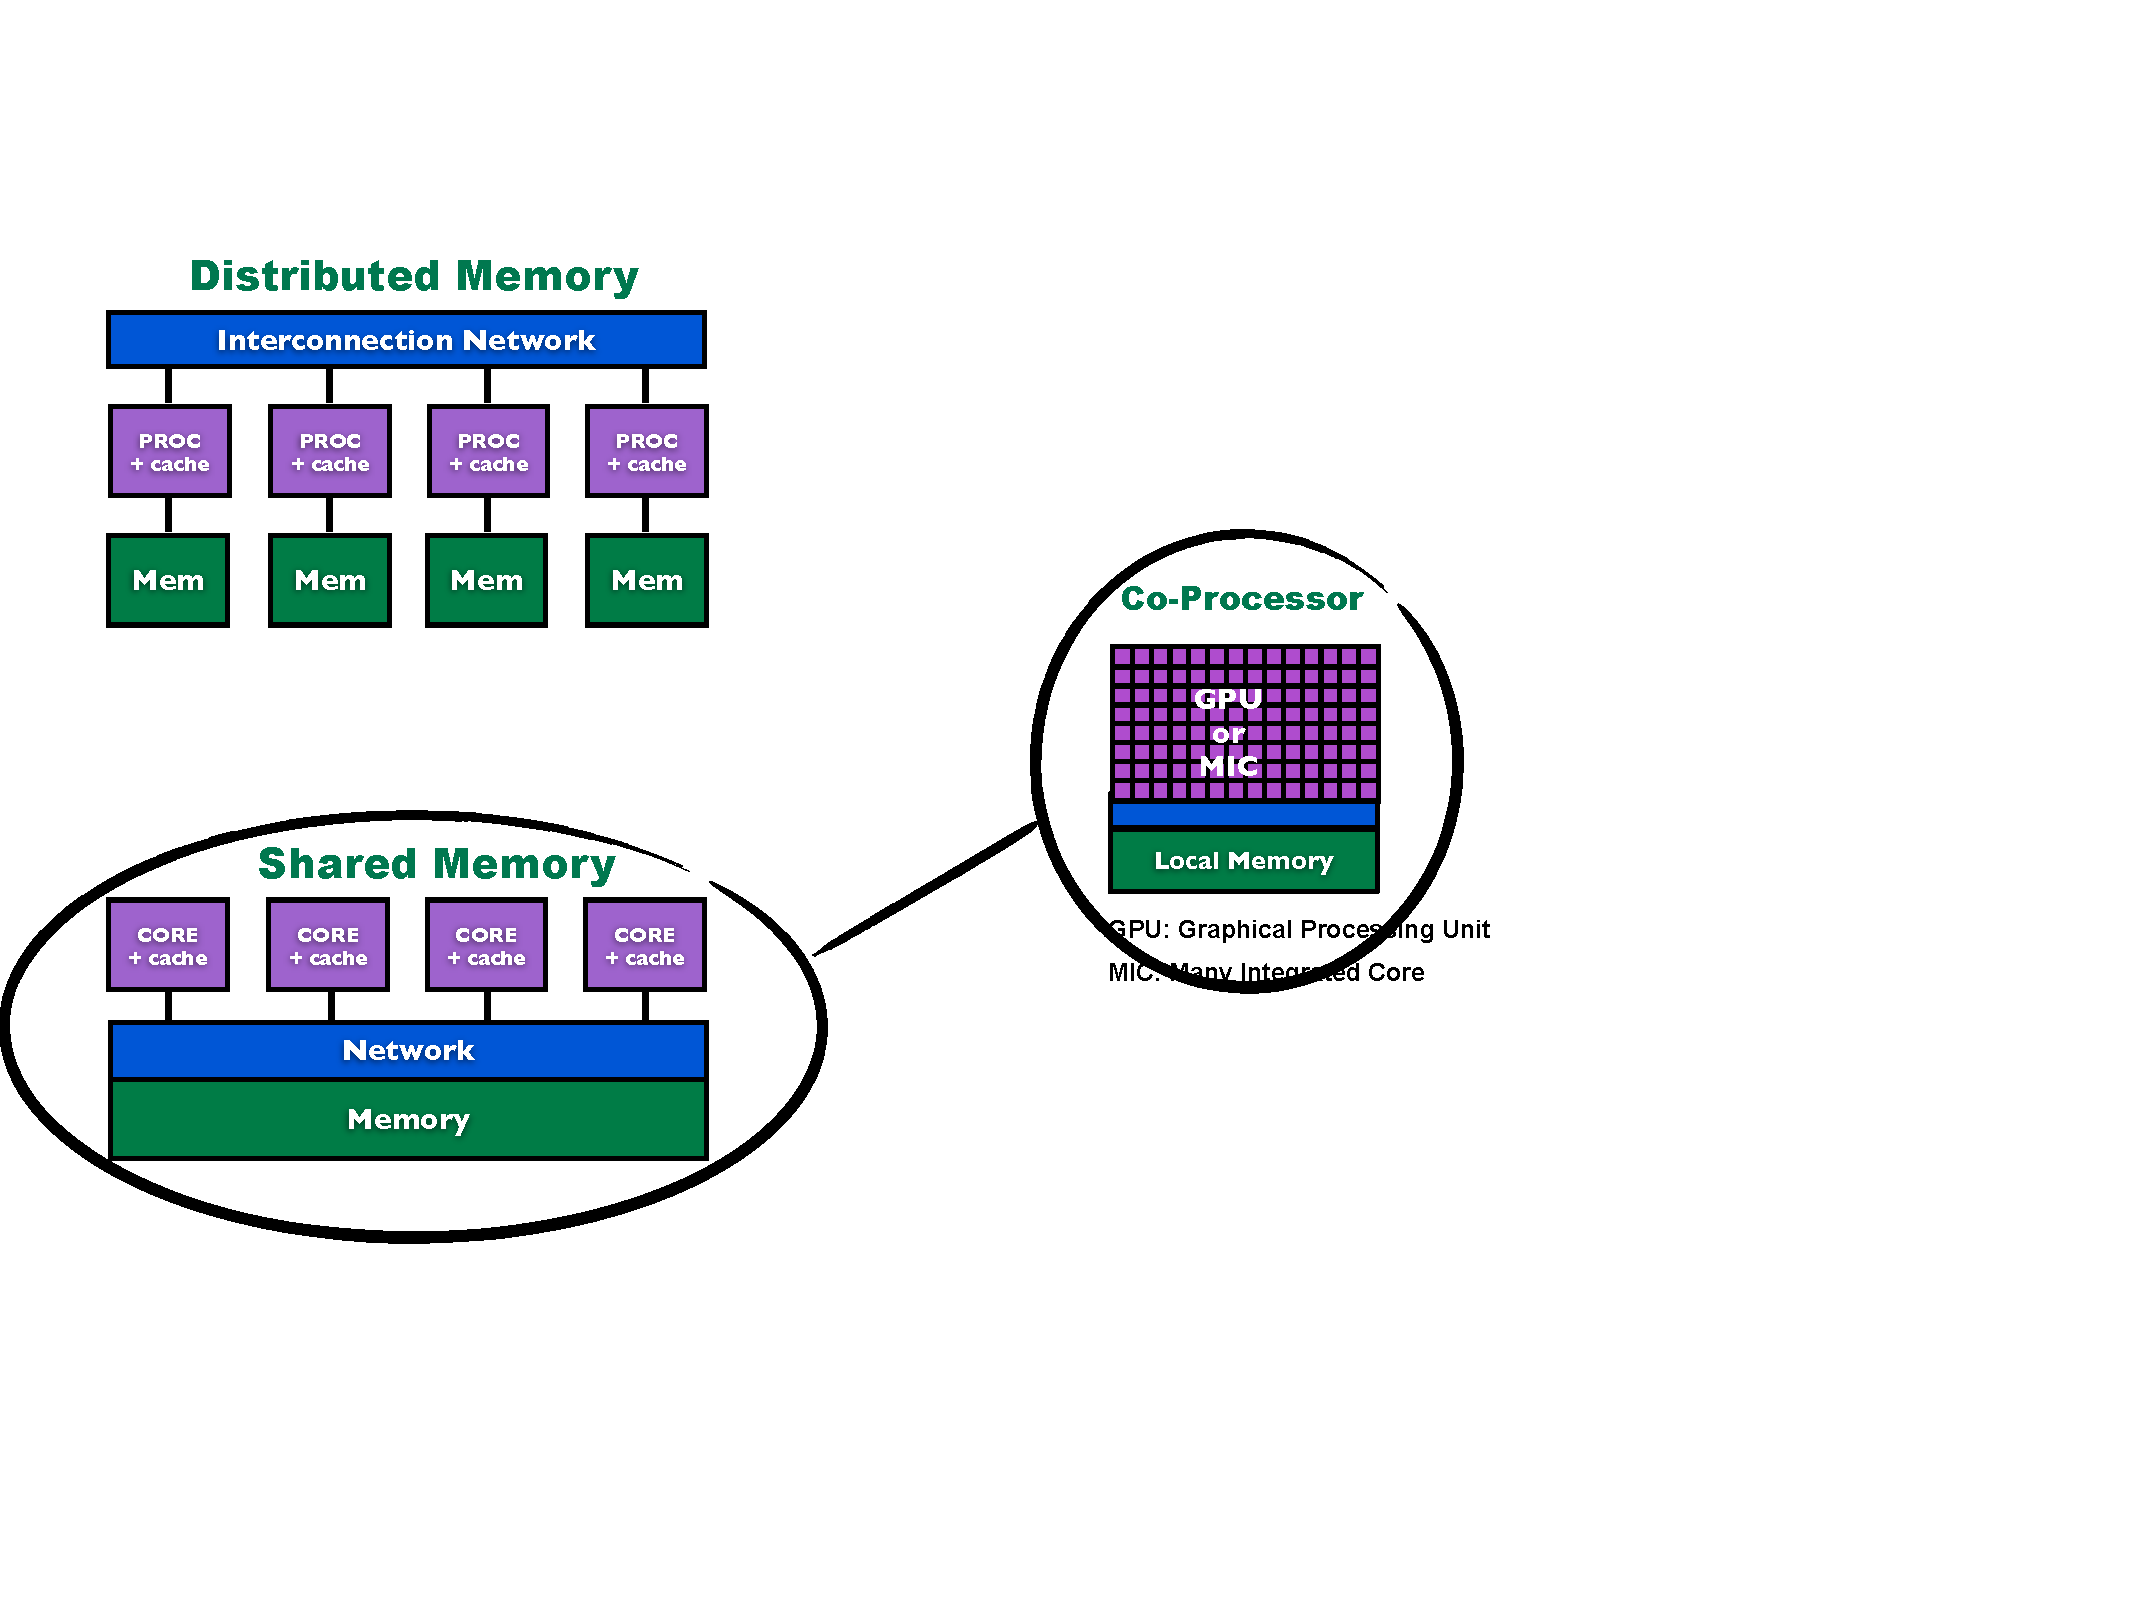
\includegraphics[width=0.95\textwidth]{../common/pics/ParallelHardware2.pdf}
\end{block}
\end{frame}

\begin{frame}
\begin{block}{A Server or Cluster}
    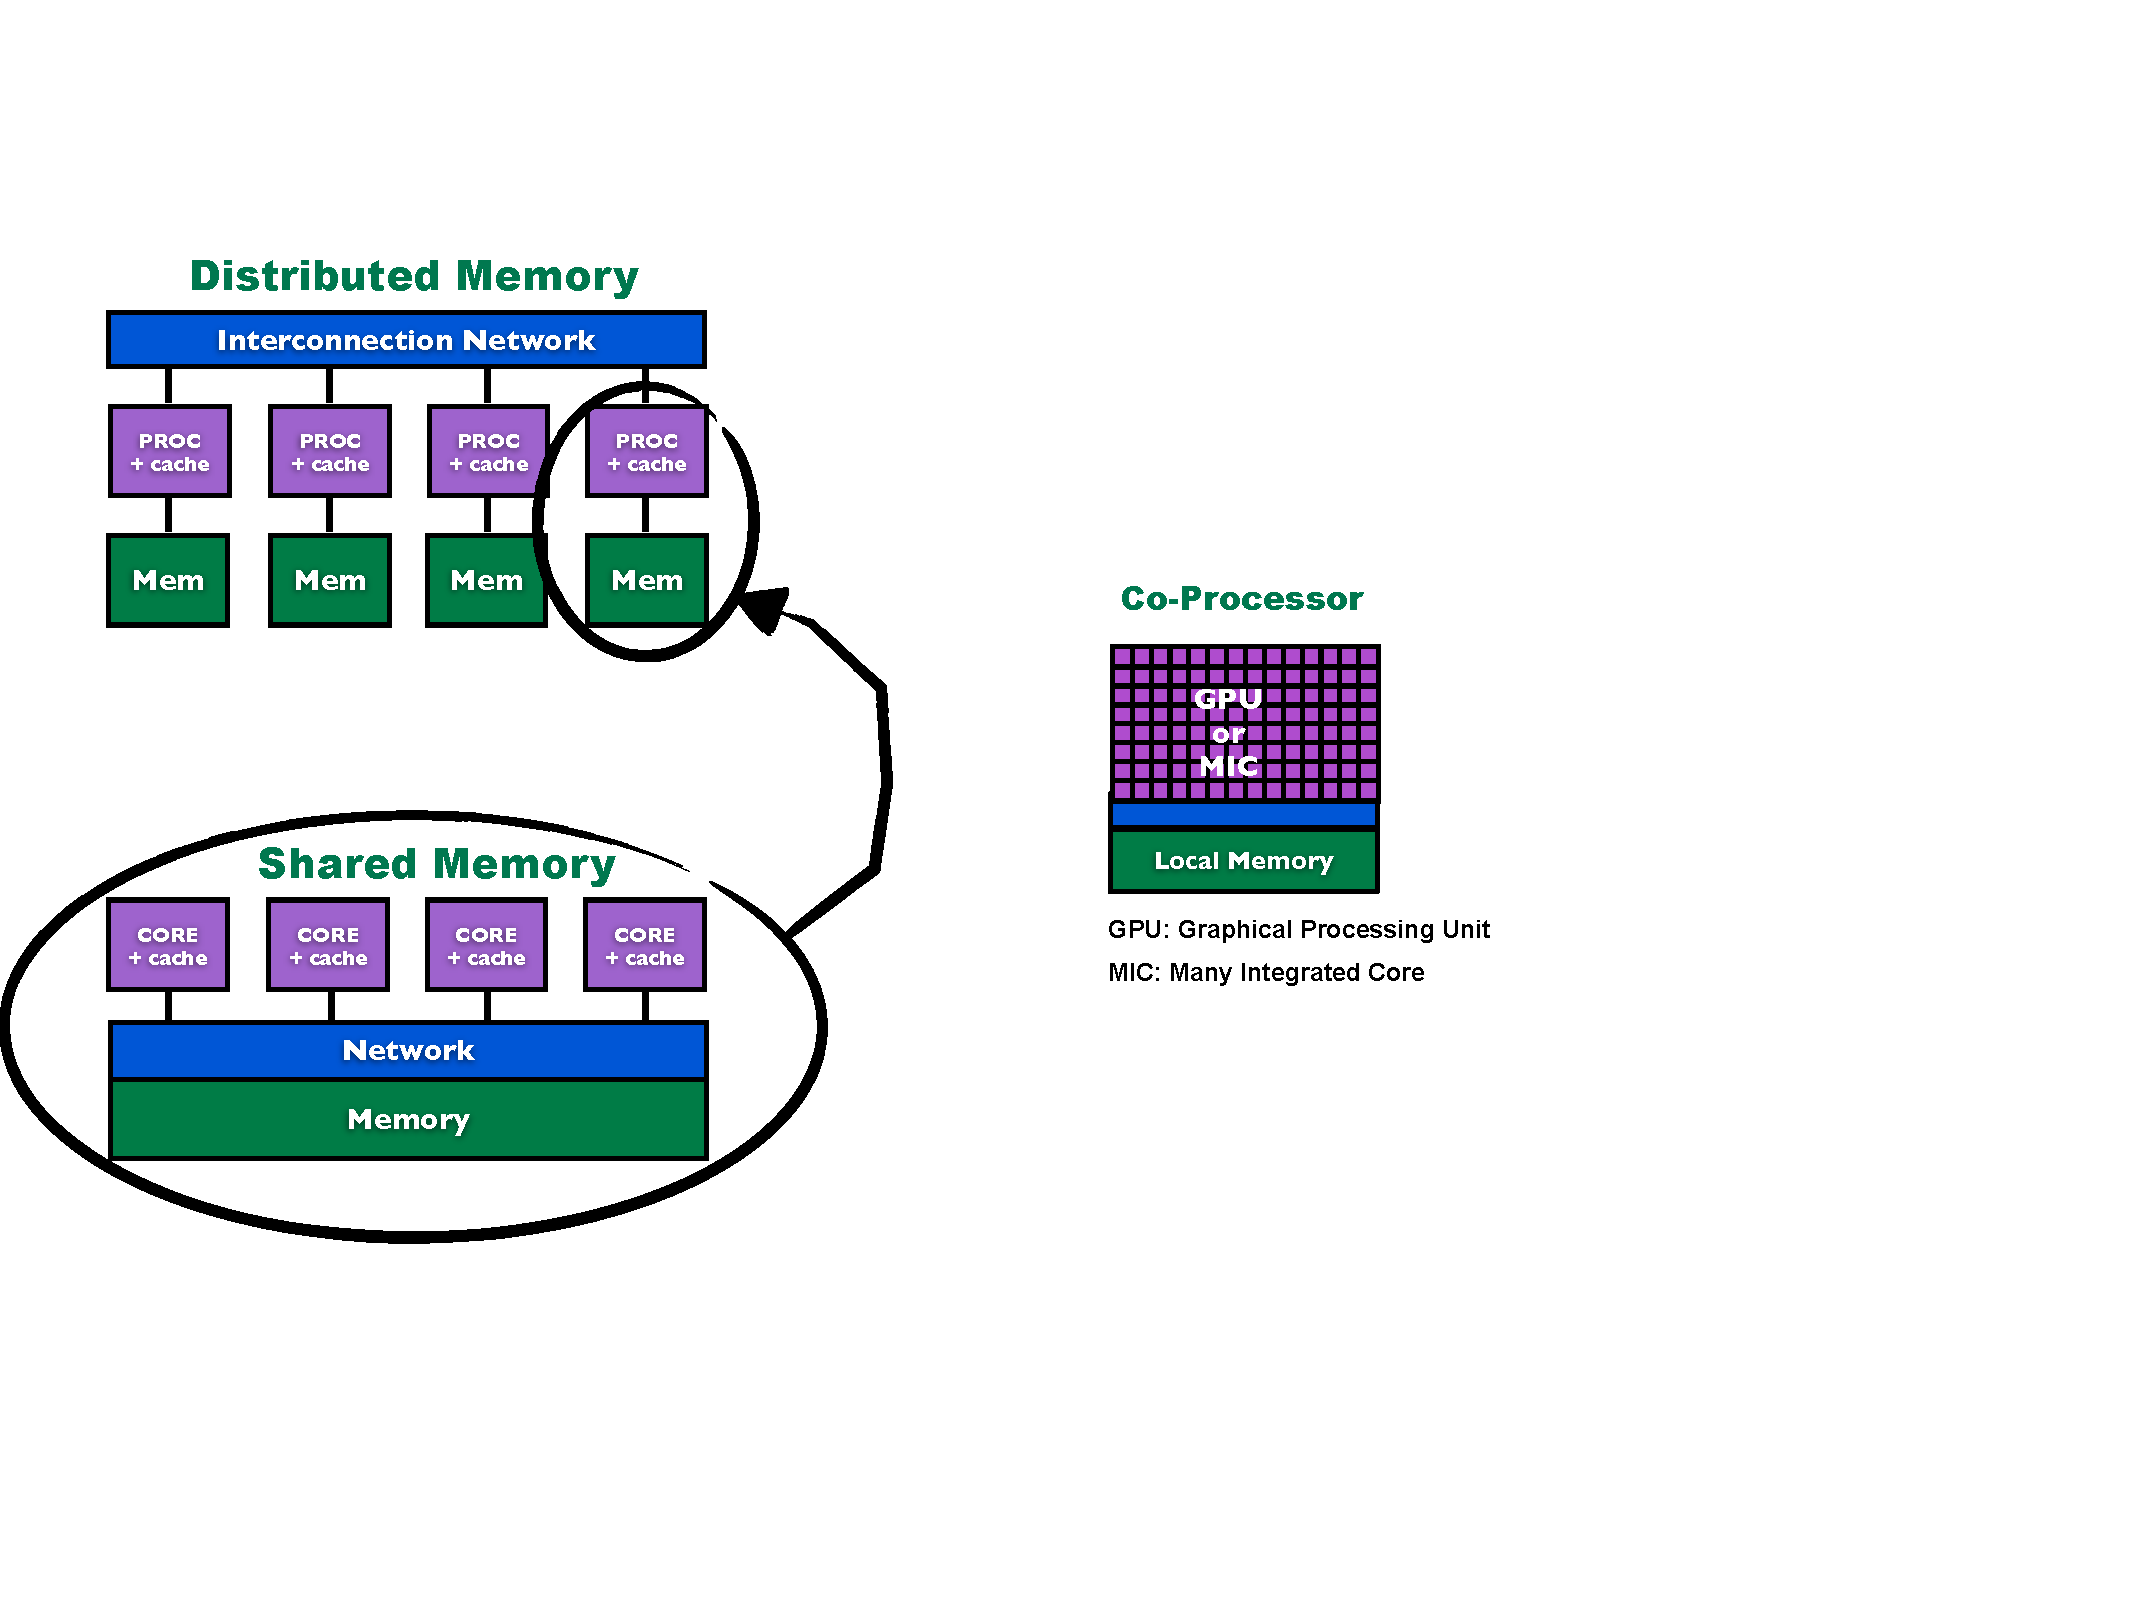
\includegraphics[width=0.95\textwidth]{../common/pics/ParallelHardware3.pdf}
\end{block}
\end{frame}

\begin{frame}
\begin{block}{Server to Supercomputer}
    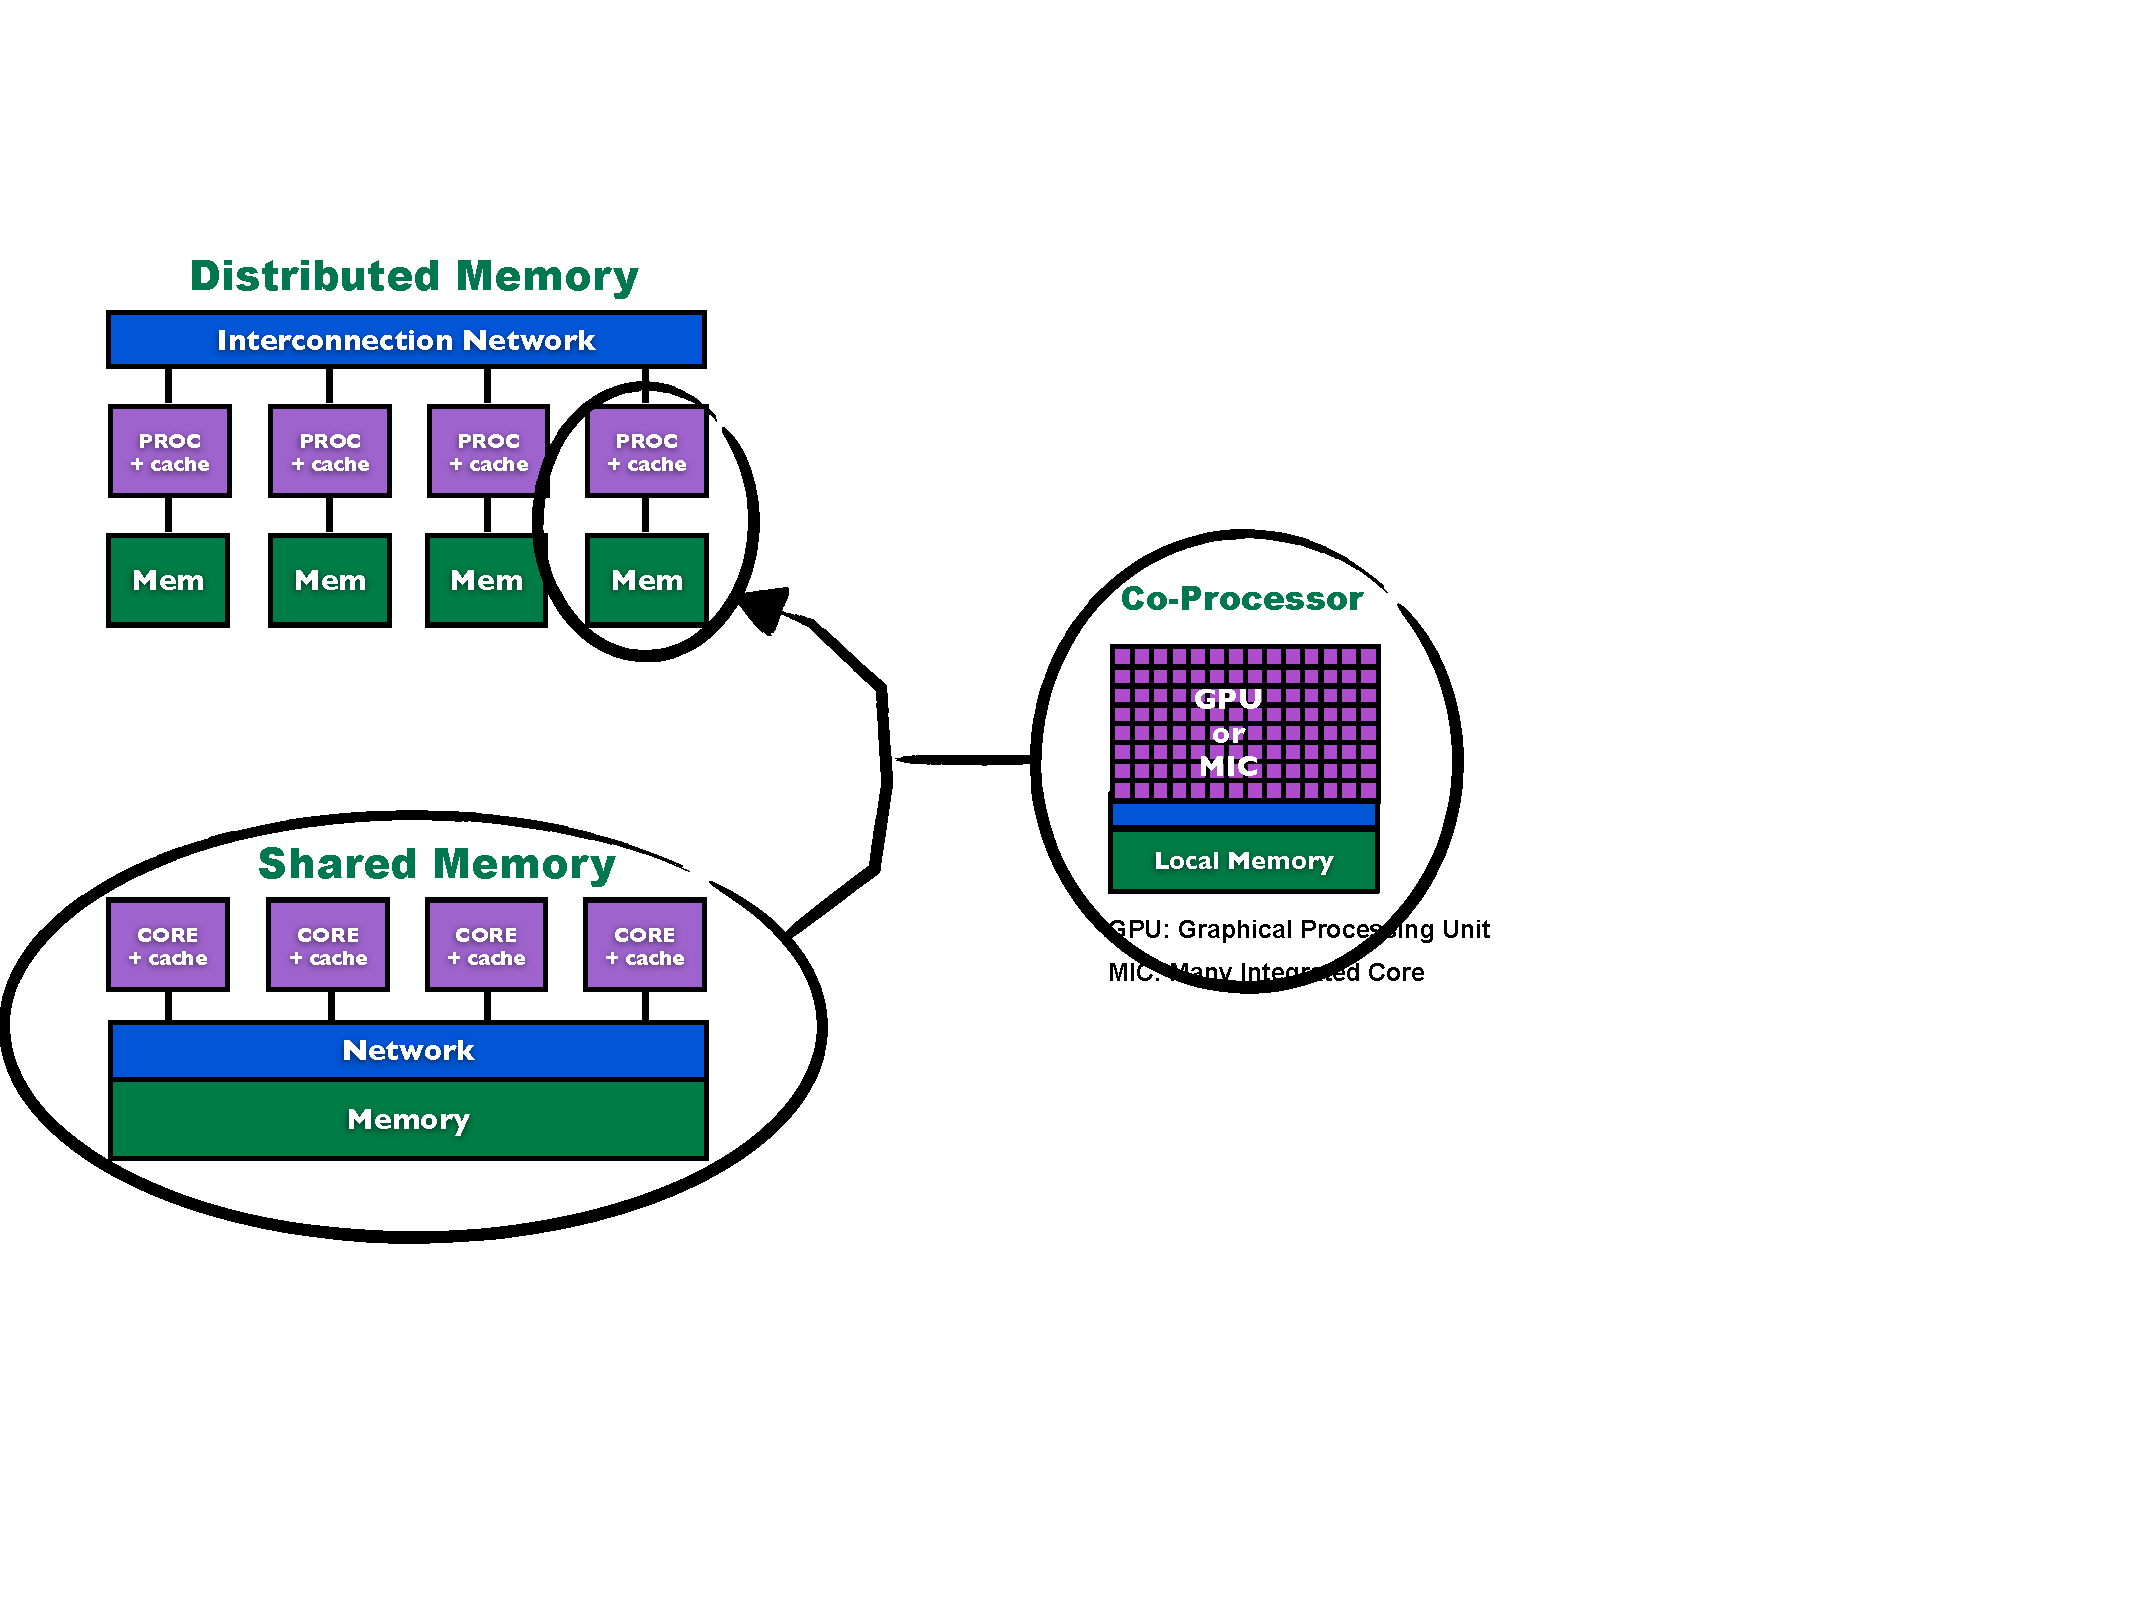
\includegraphics[width=0.95\textwidth]{../common/pics/ParallelHardware4.pdf}
\end{block}
\end{frame}

\begin{frame}
\begin{block}{Knowing the Right Words}
    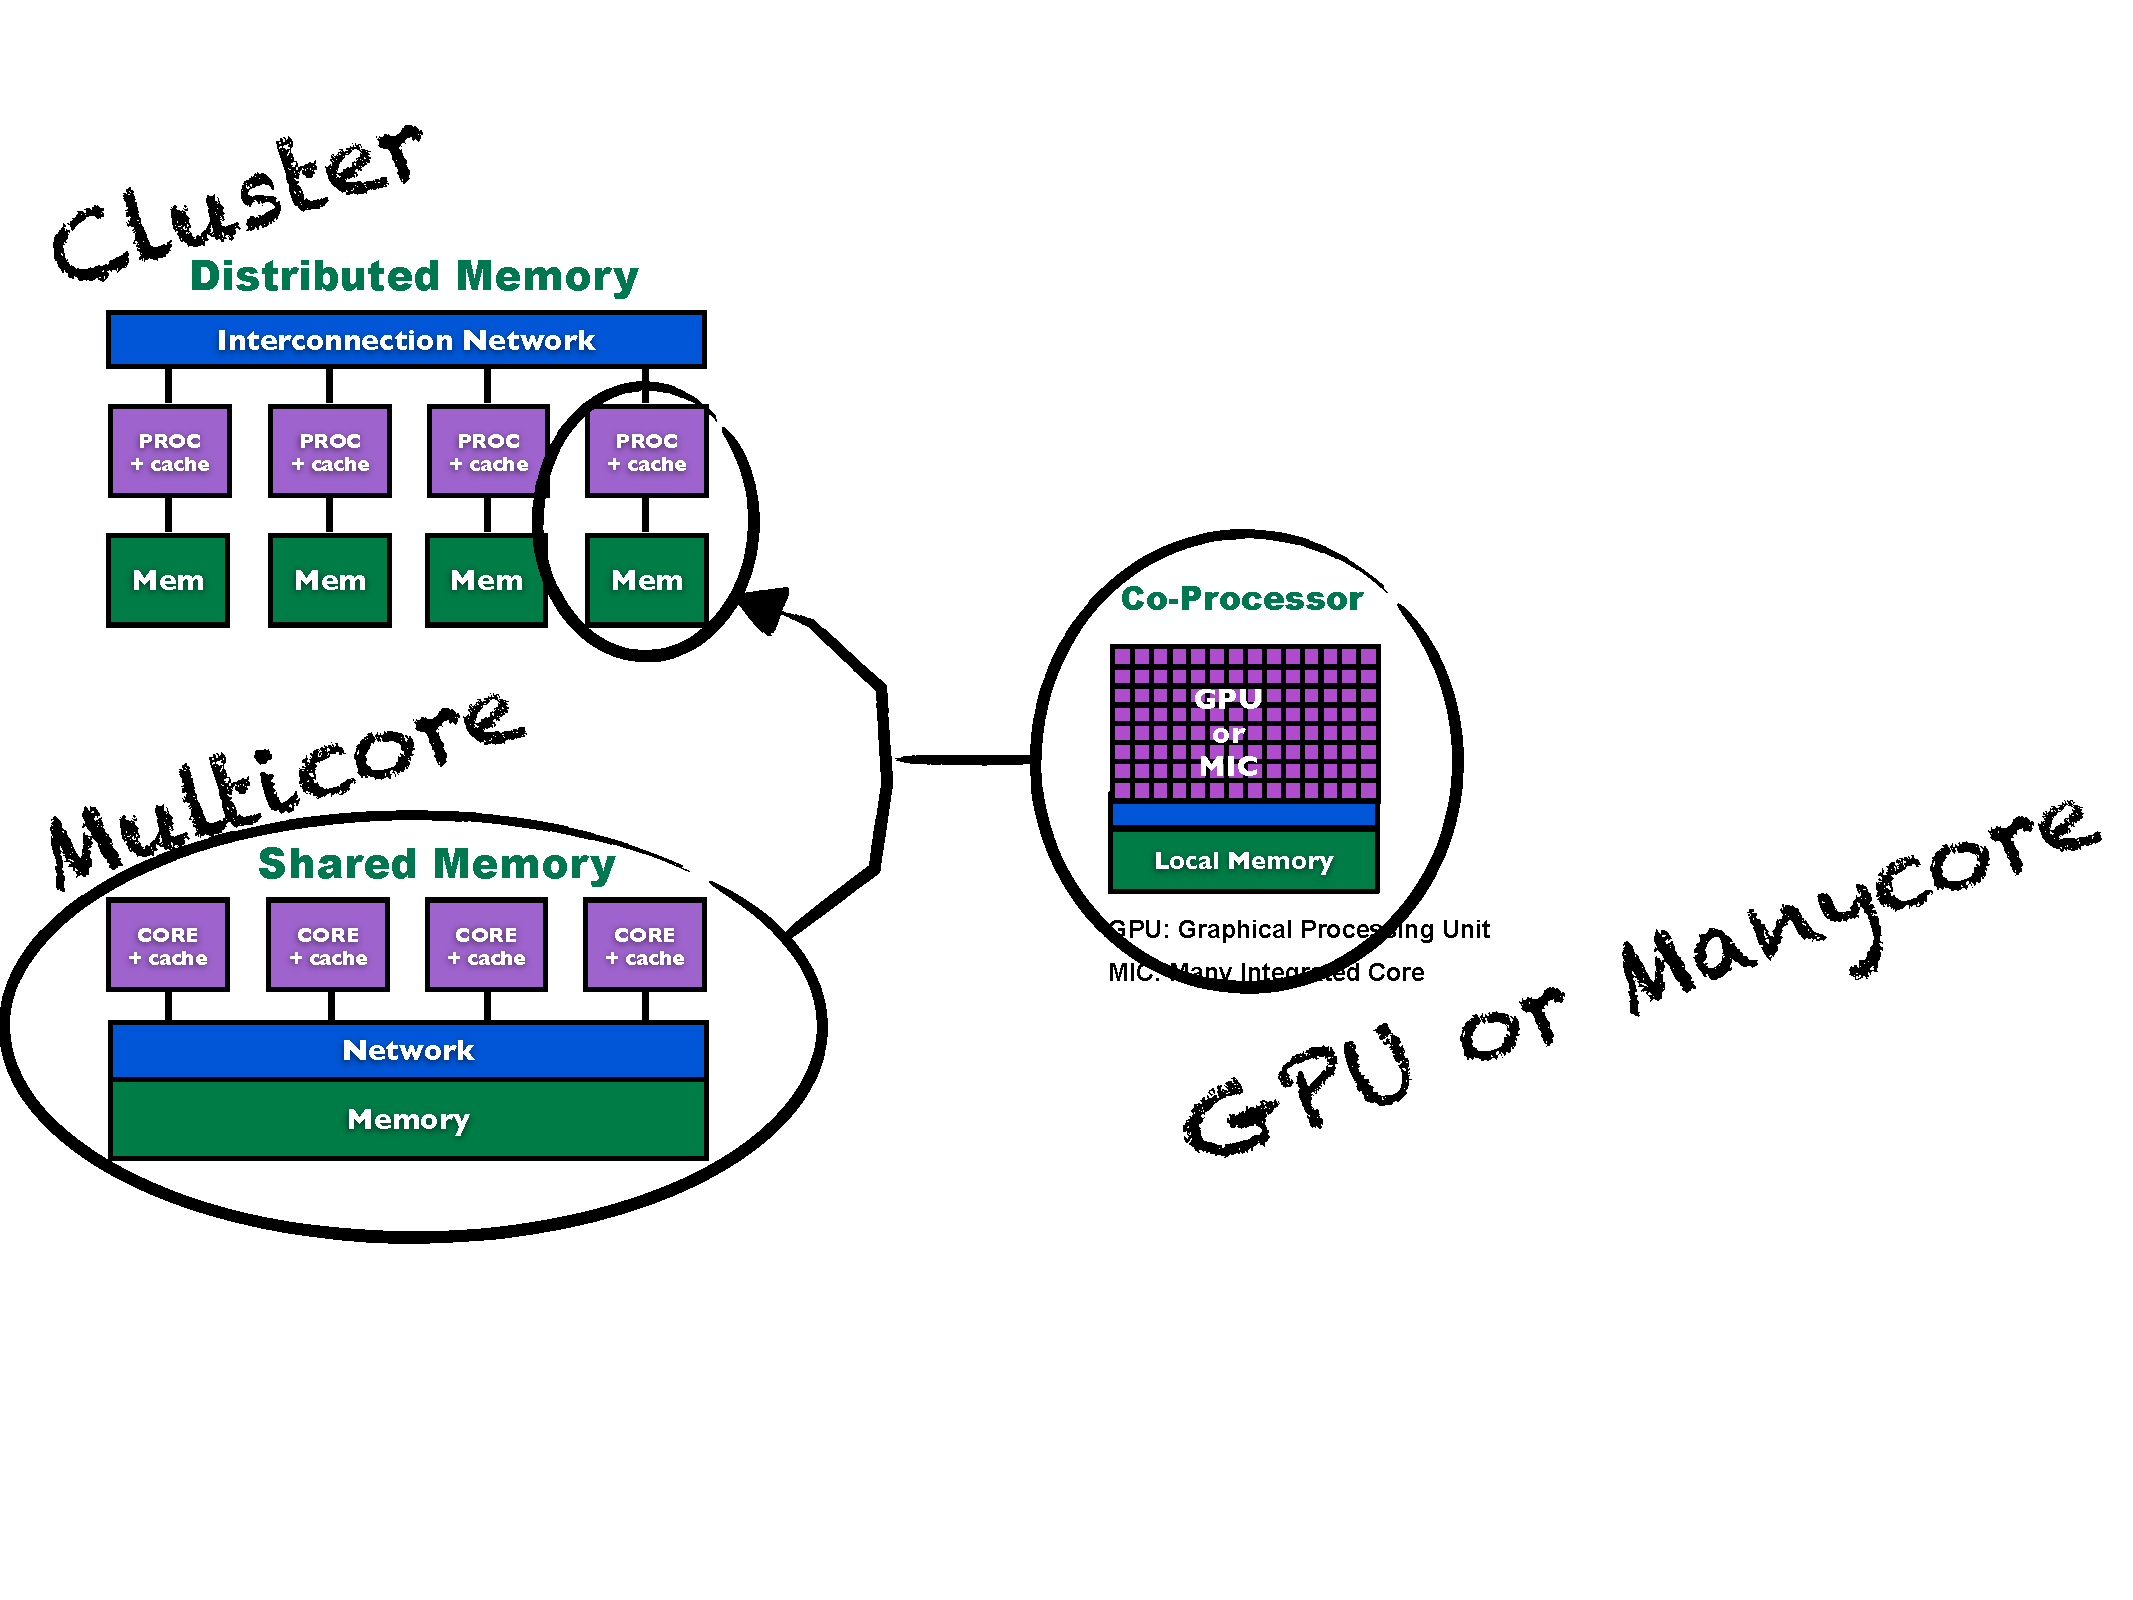
\includegraphics[width=0.95\textwidth]{../common/pics/ParallelHardware5.pdf}
\end{block}
\end{frame}

\begin{frame}
\begin{block}{``Native'' Programming Models and Tools}
    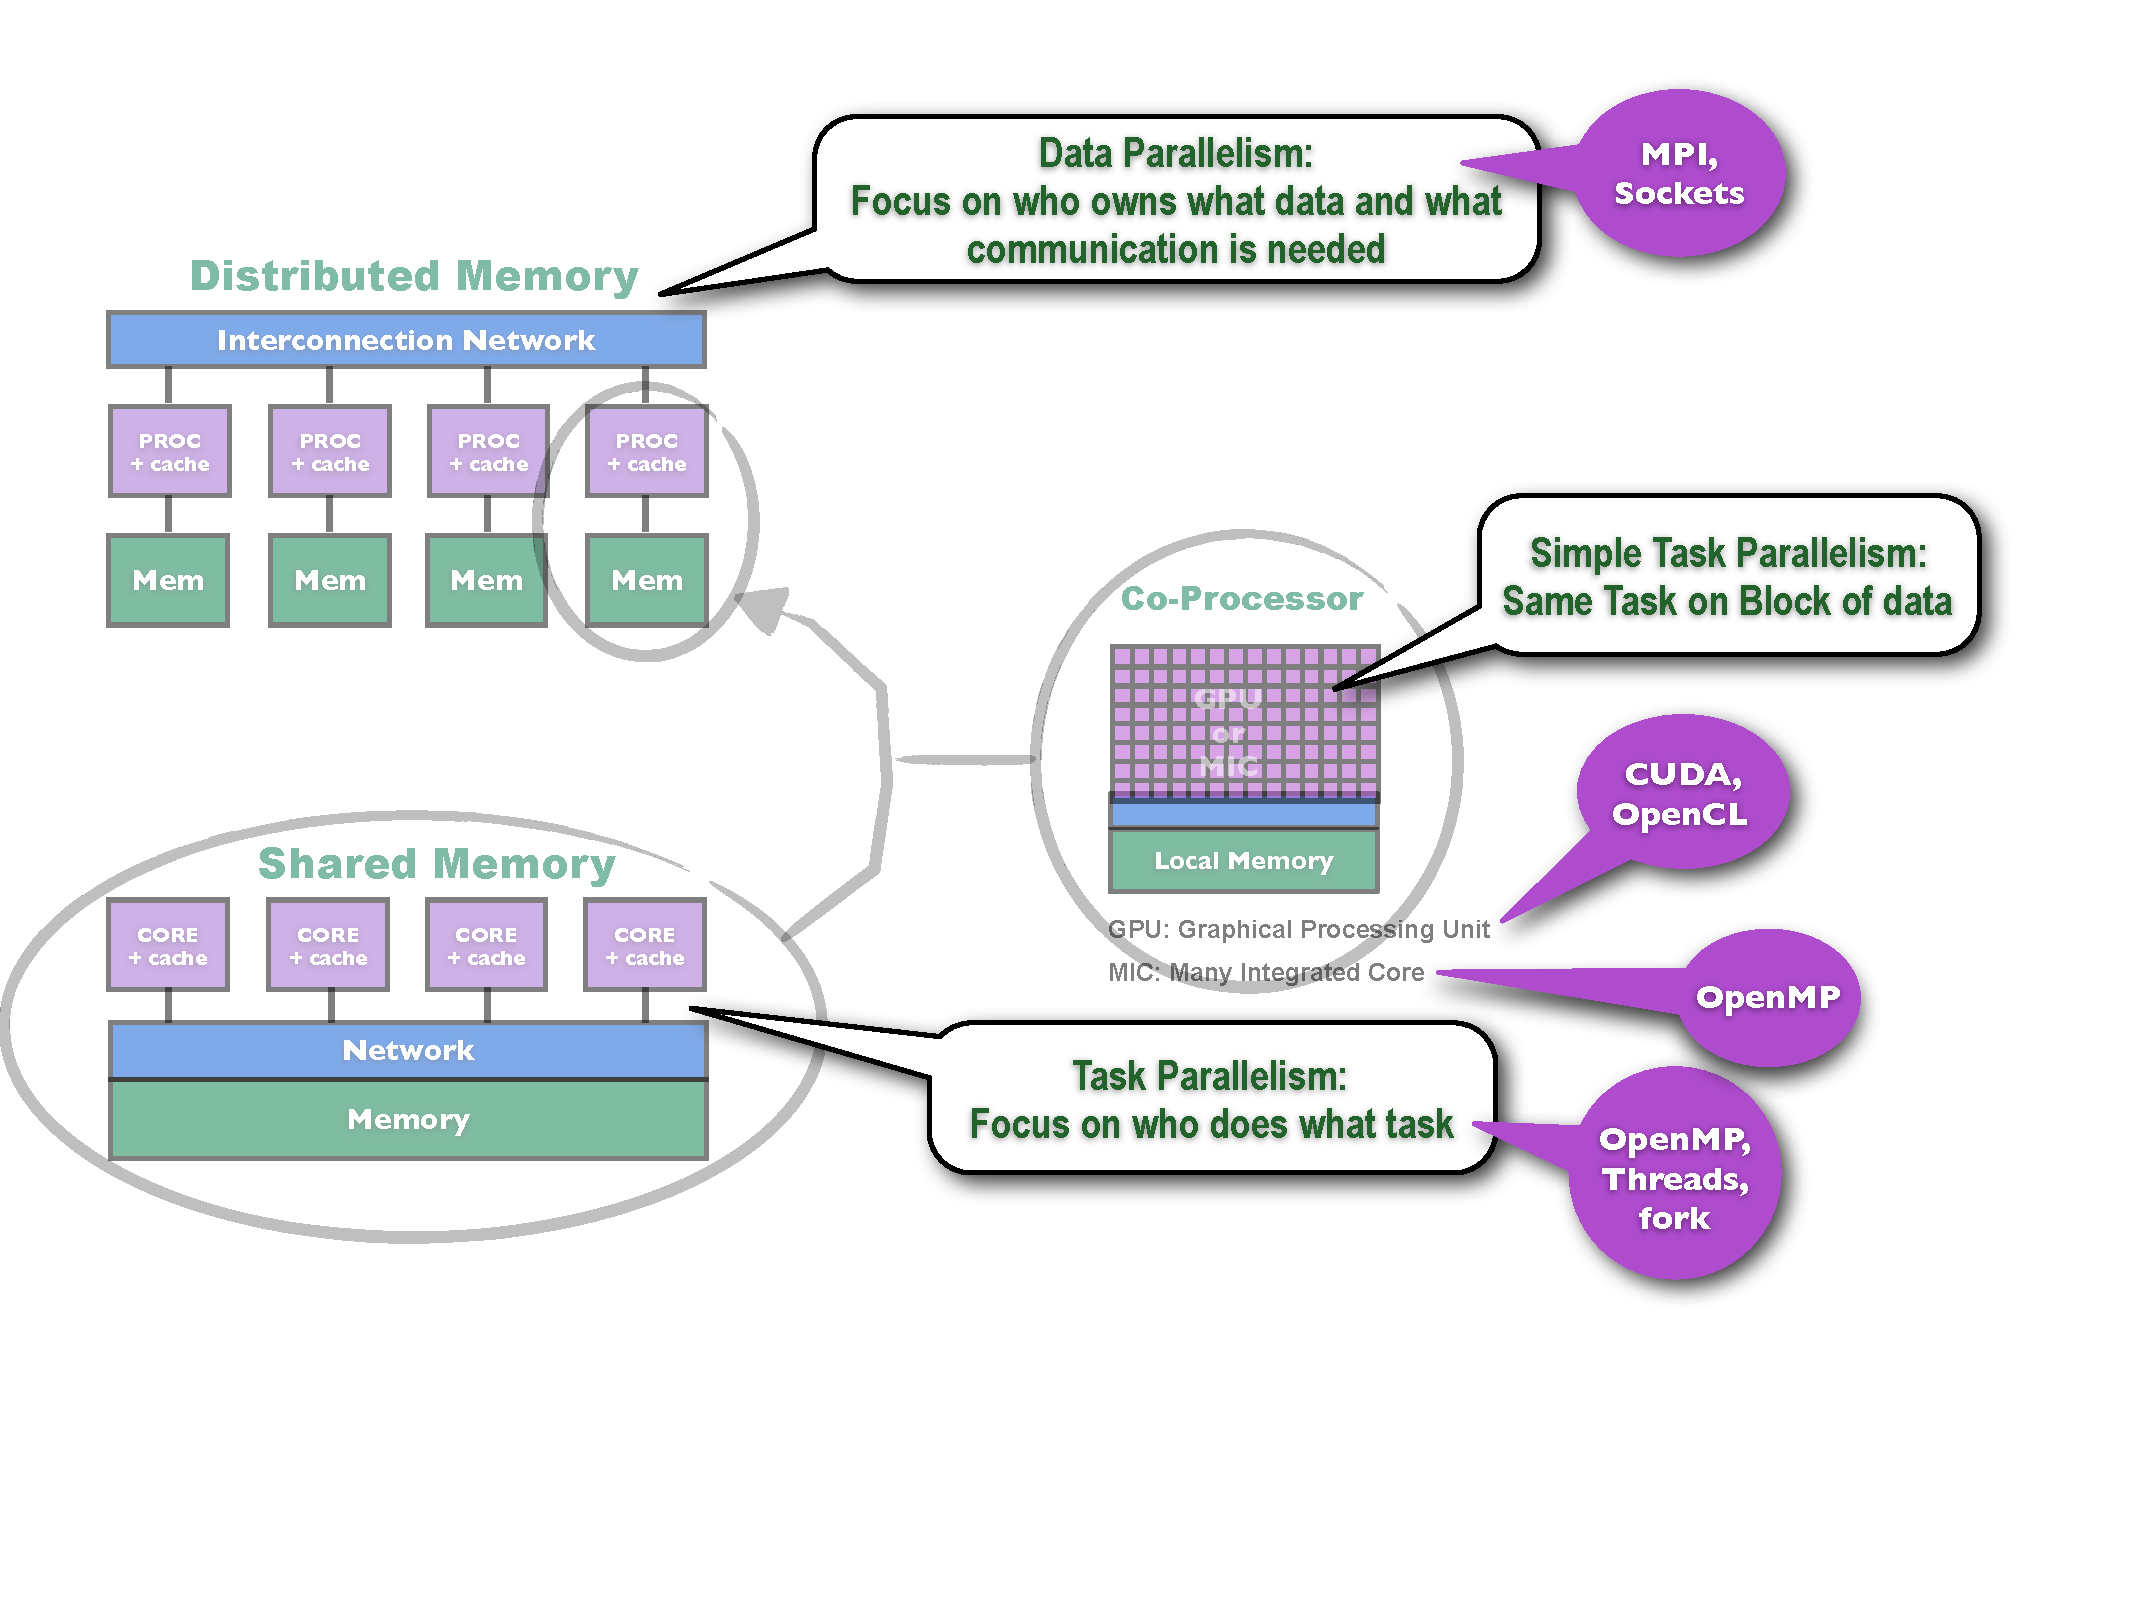
\includegraphics[width=0.95\textwidth]{../common/pics/ParallelHardware6.pdf}
\end{block}
\end{frame}

\begin{frame}
\begin{block}{R Interfaces to Native Tools}
    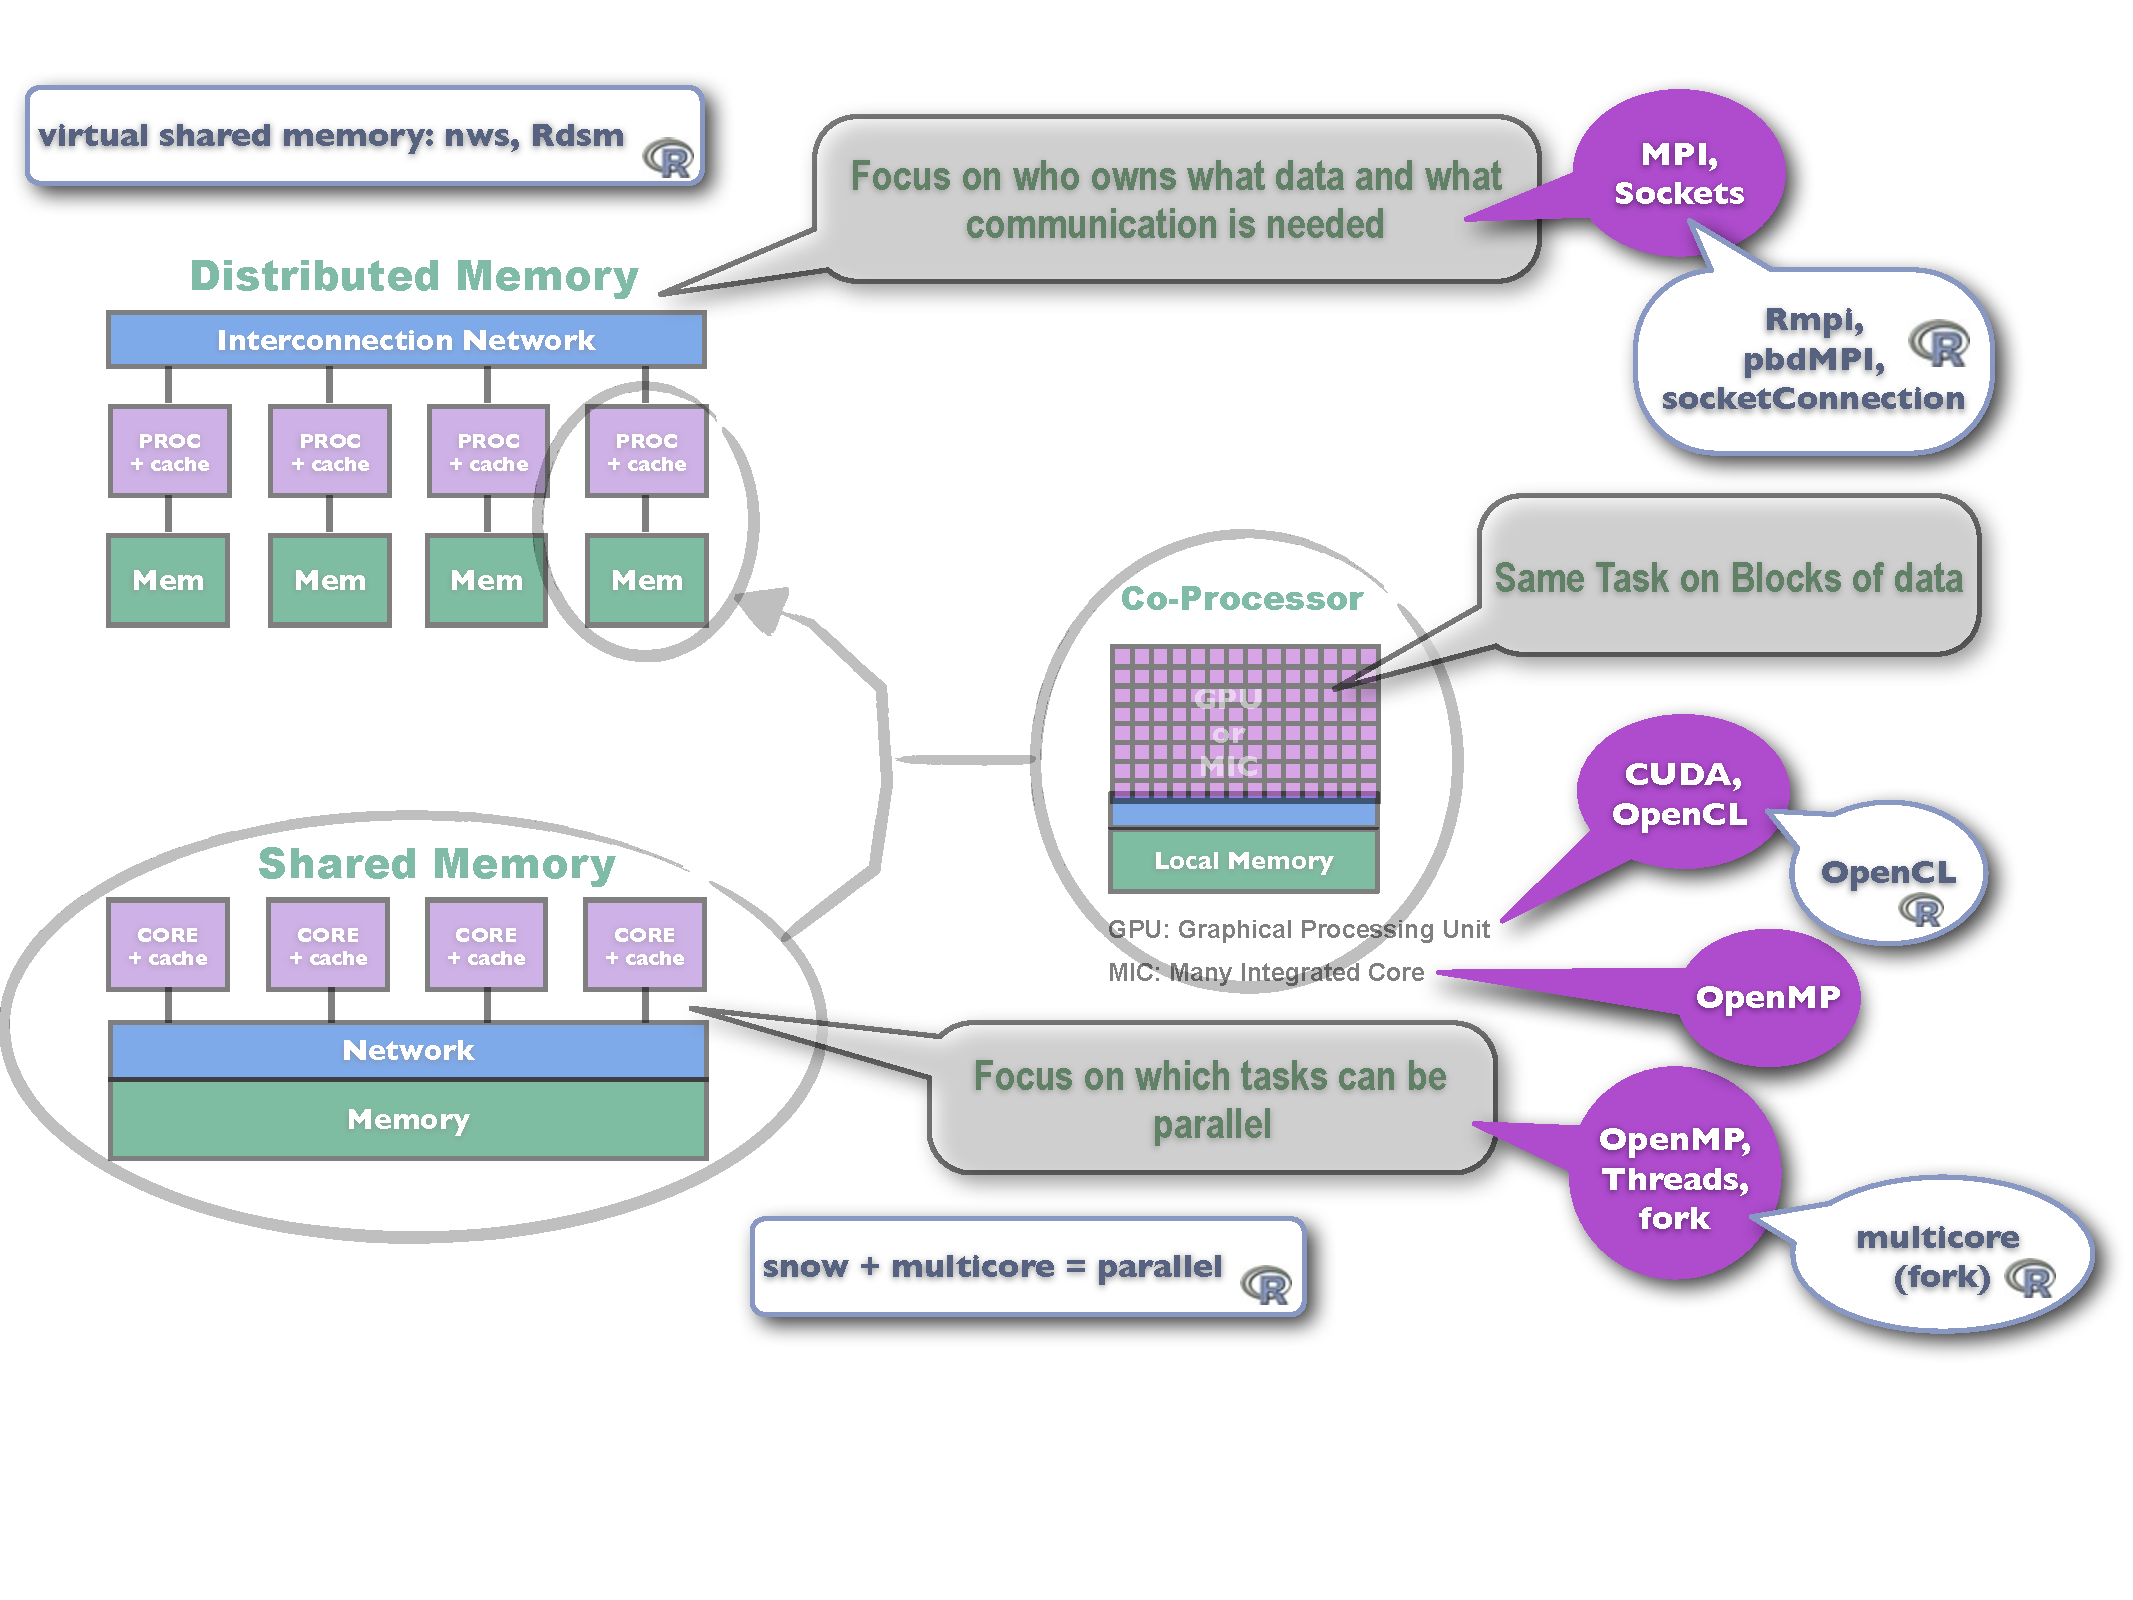
\includegraphics[width=0.95\textwidth]{../common/pics/ParallelHardware7.pdf}
\end{block}
\end{frame}

\begin{frame}
\begin{block}{30+ Years of Parallel Computing Research}
    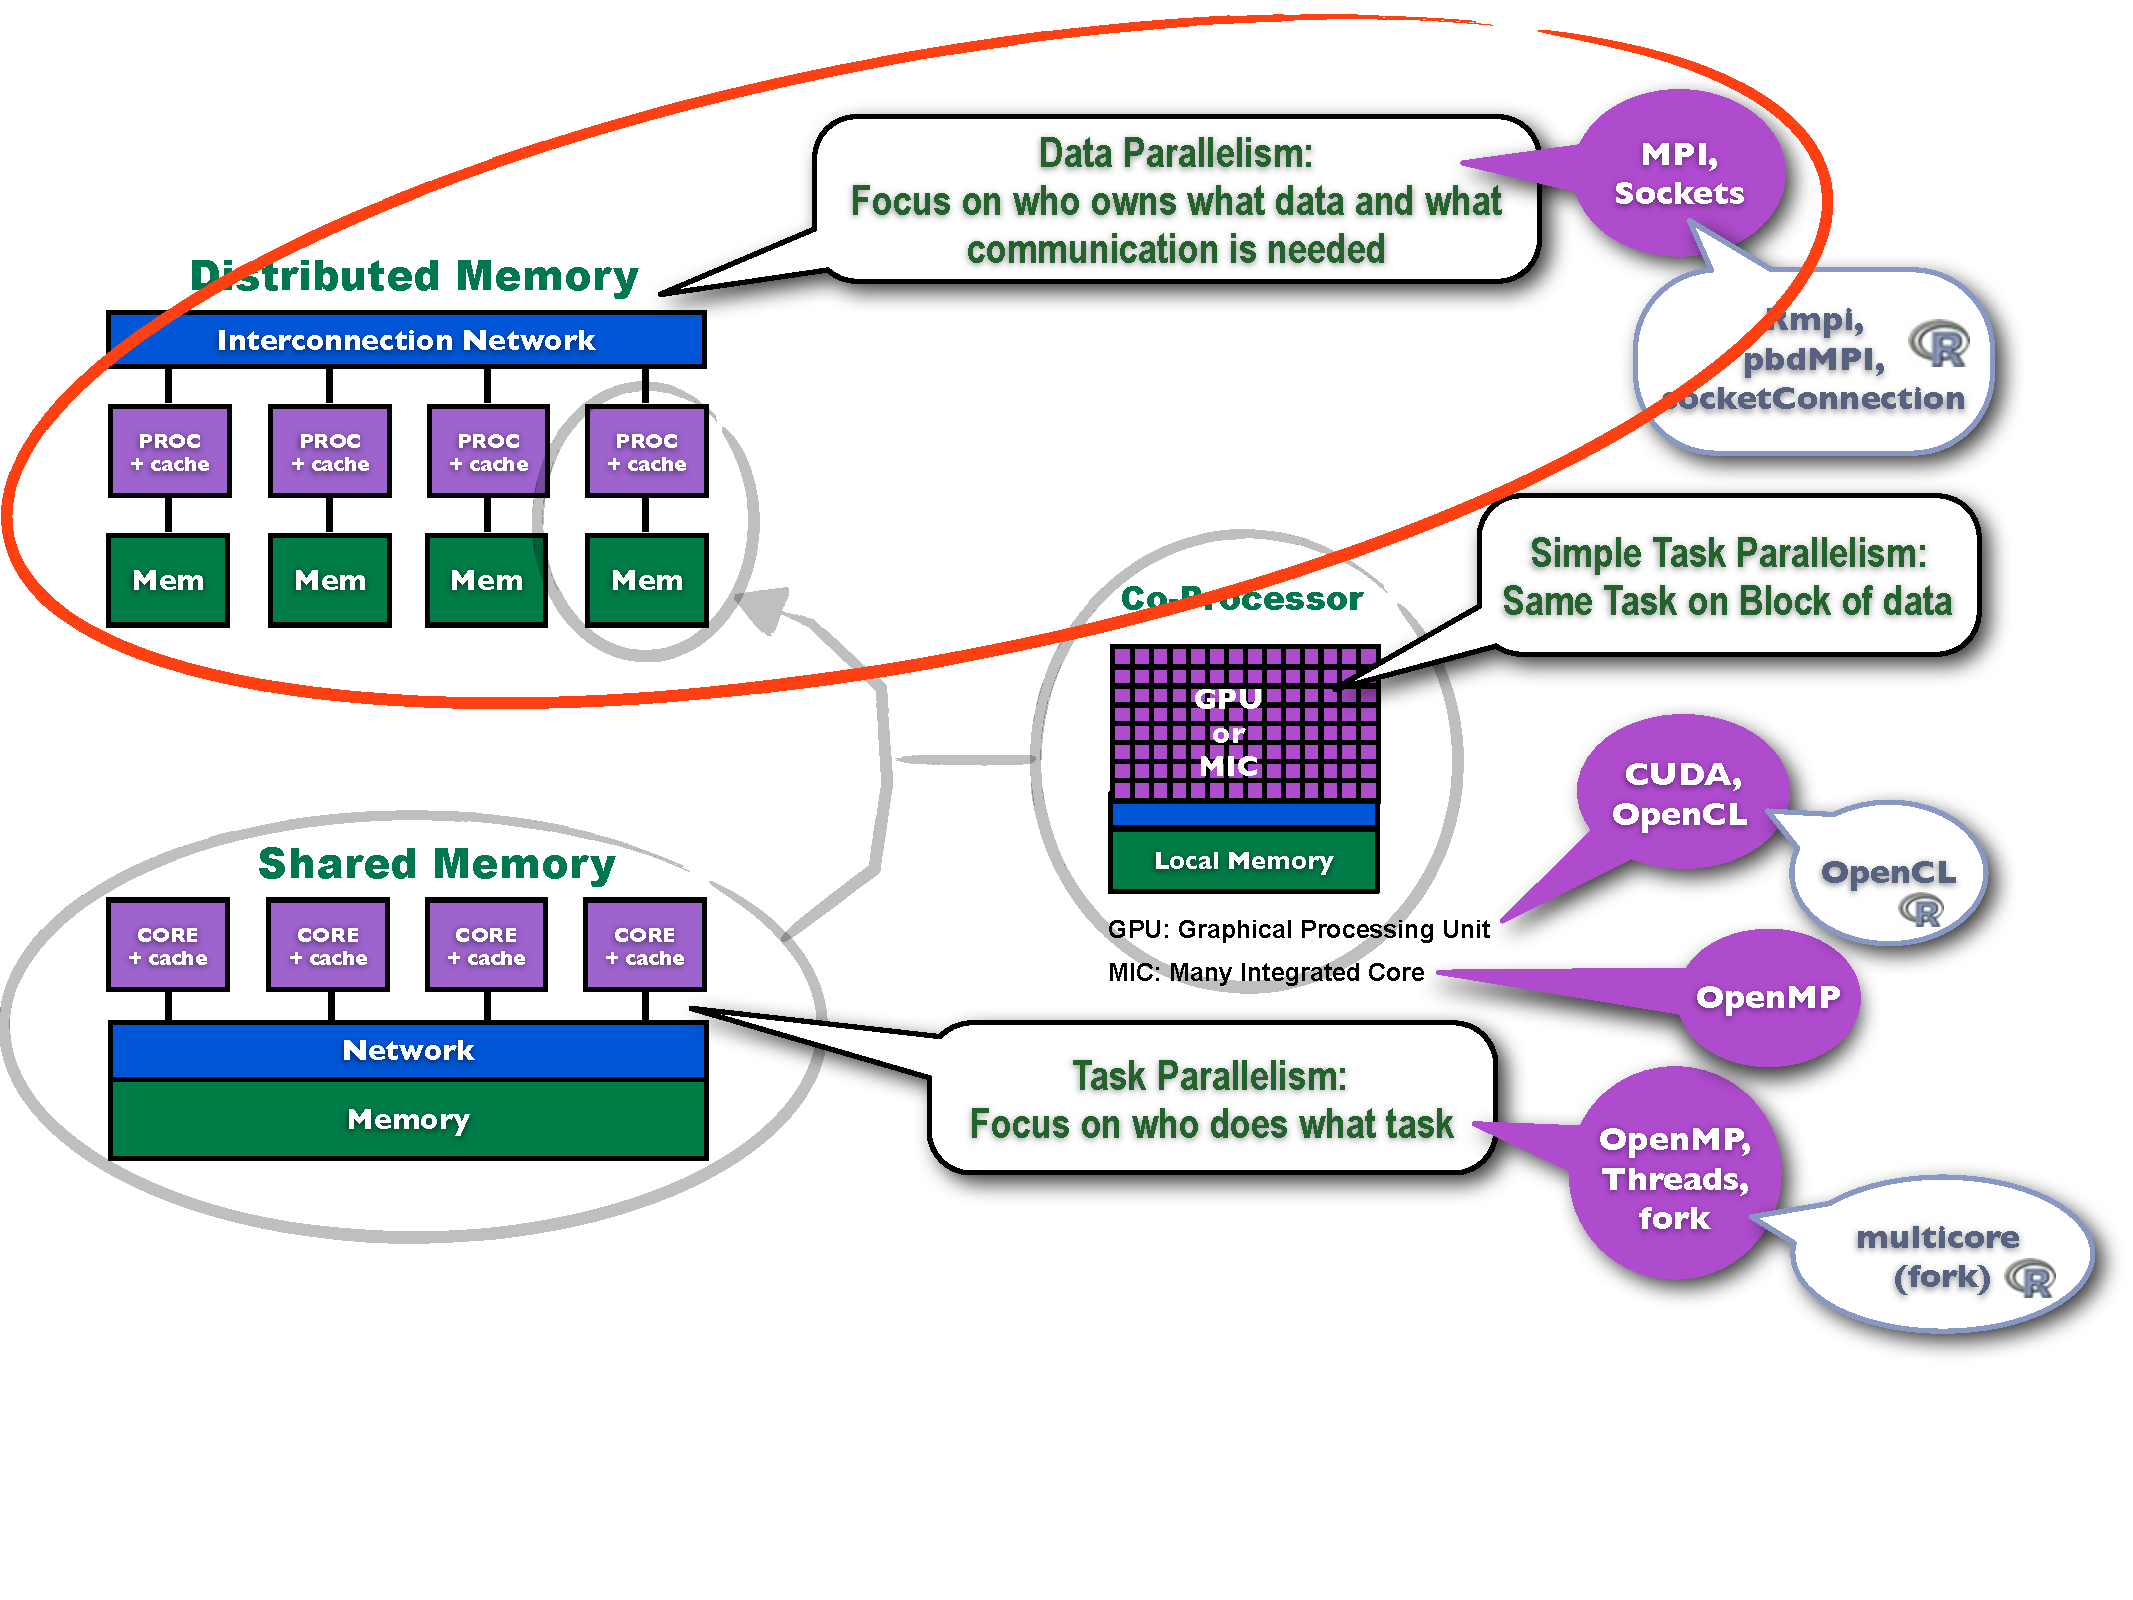
\includegraphics[width=0.95\textwidth]{../common/pics/ParallelHardware8.pdf}
\end{block}
\end{frame}

\begin{frame}
\begin{block}{Last 10 years of Advances}
    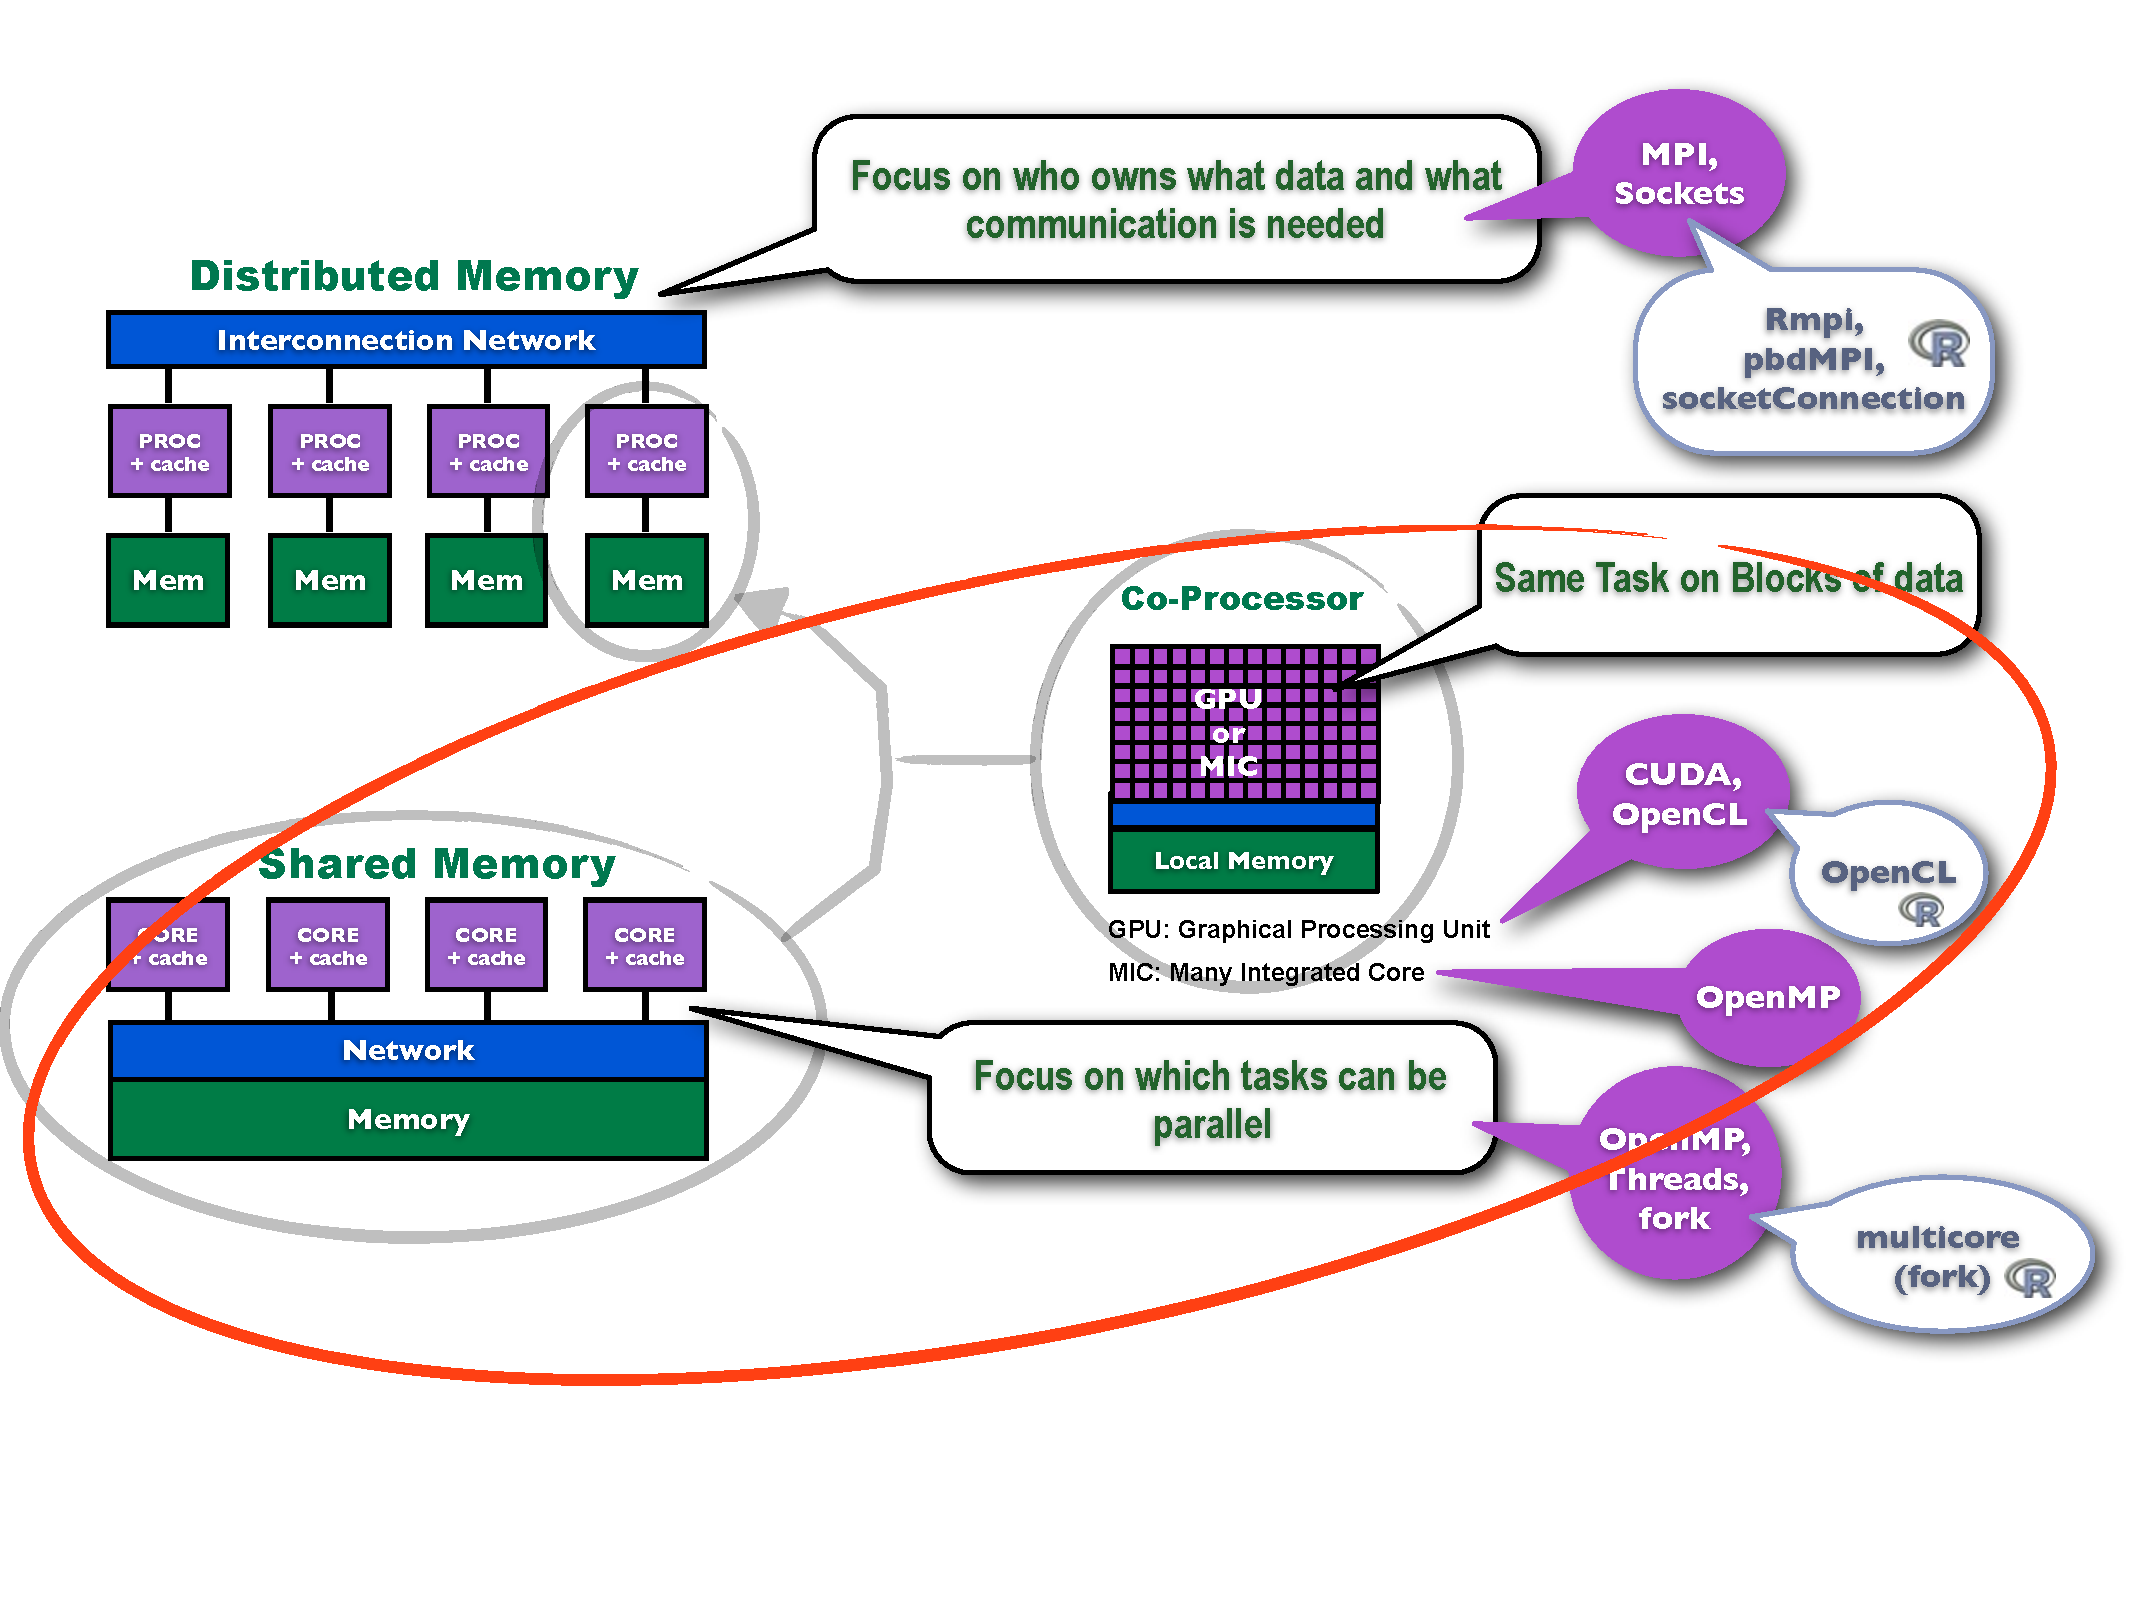
\includegraphics[width=0.95\textwidth]{../common/pics/ParallelHardware9.pdf}
\end{block}
\end{frame}

\begin{frame}
\begin{block}{Putting It All Together Challenge}
    
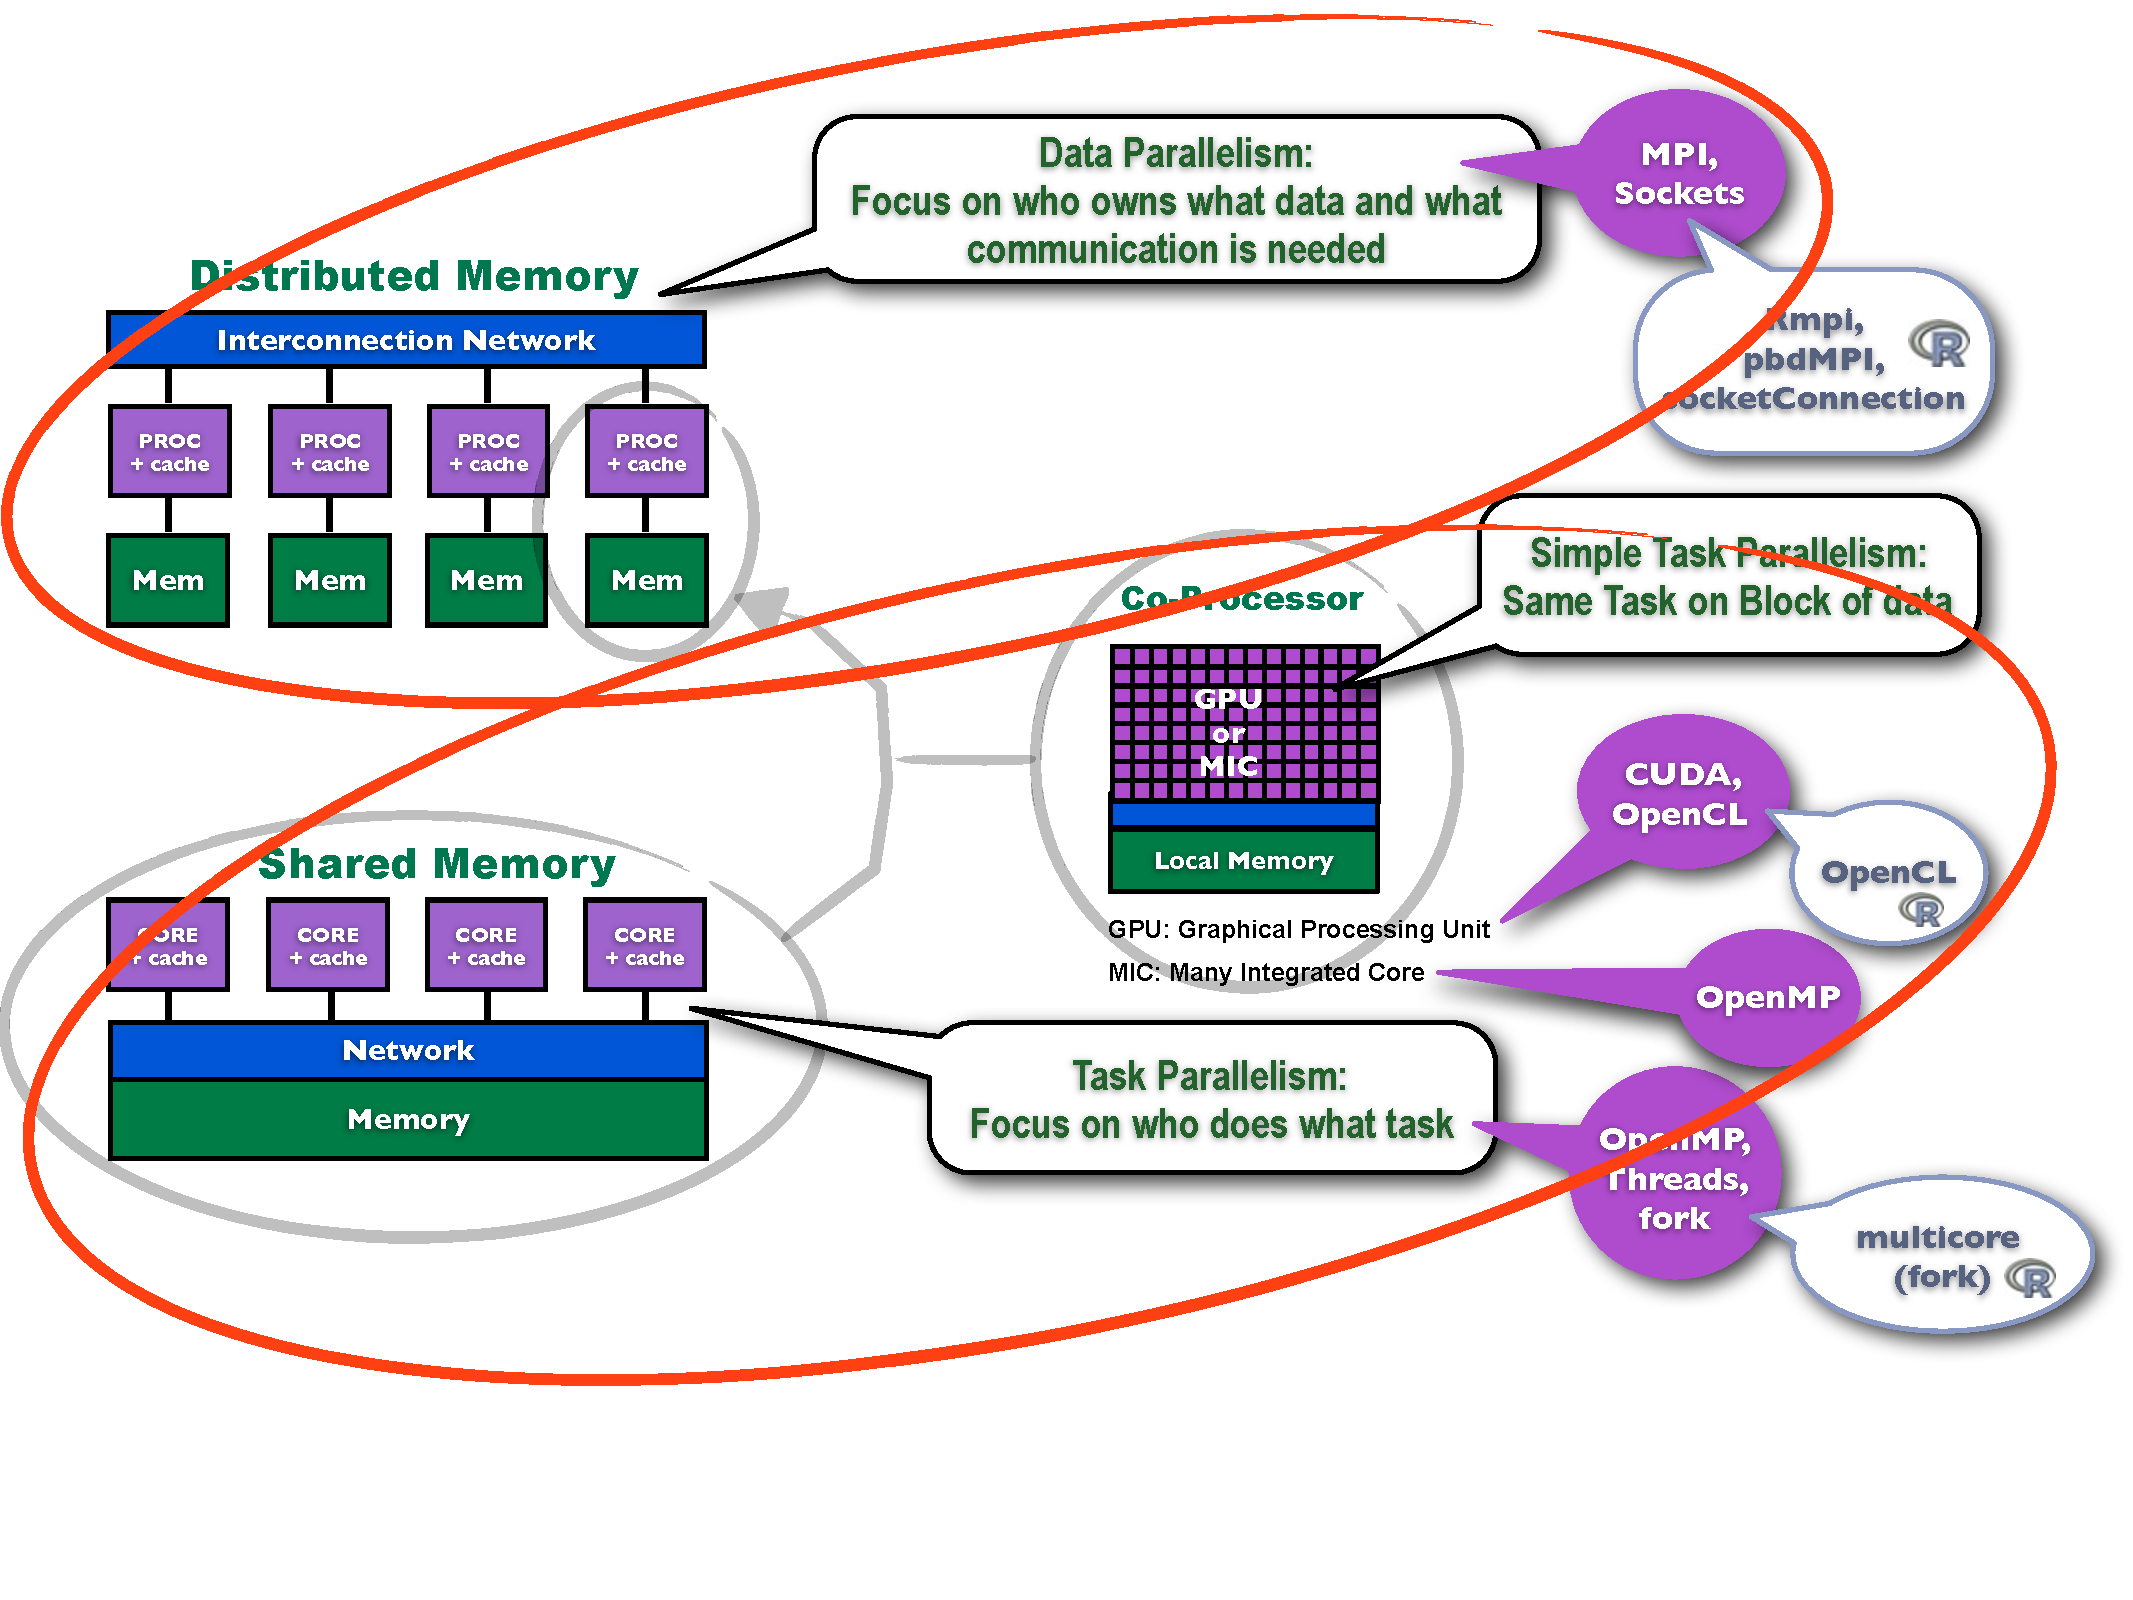
\includegraphics[width=0.95\textwidth]{../common/pics/ParallelHardware10.pdf}
\end{block}
\end{frame}

\begin{frame}
\begin{block}{pbdR Focus on Data Parallelism}
    
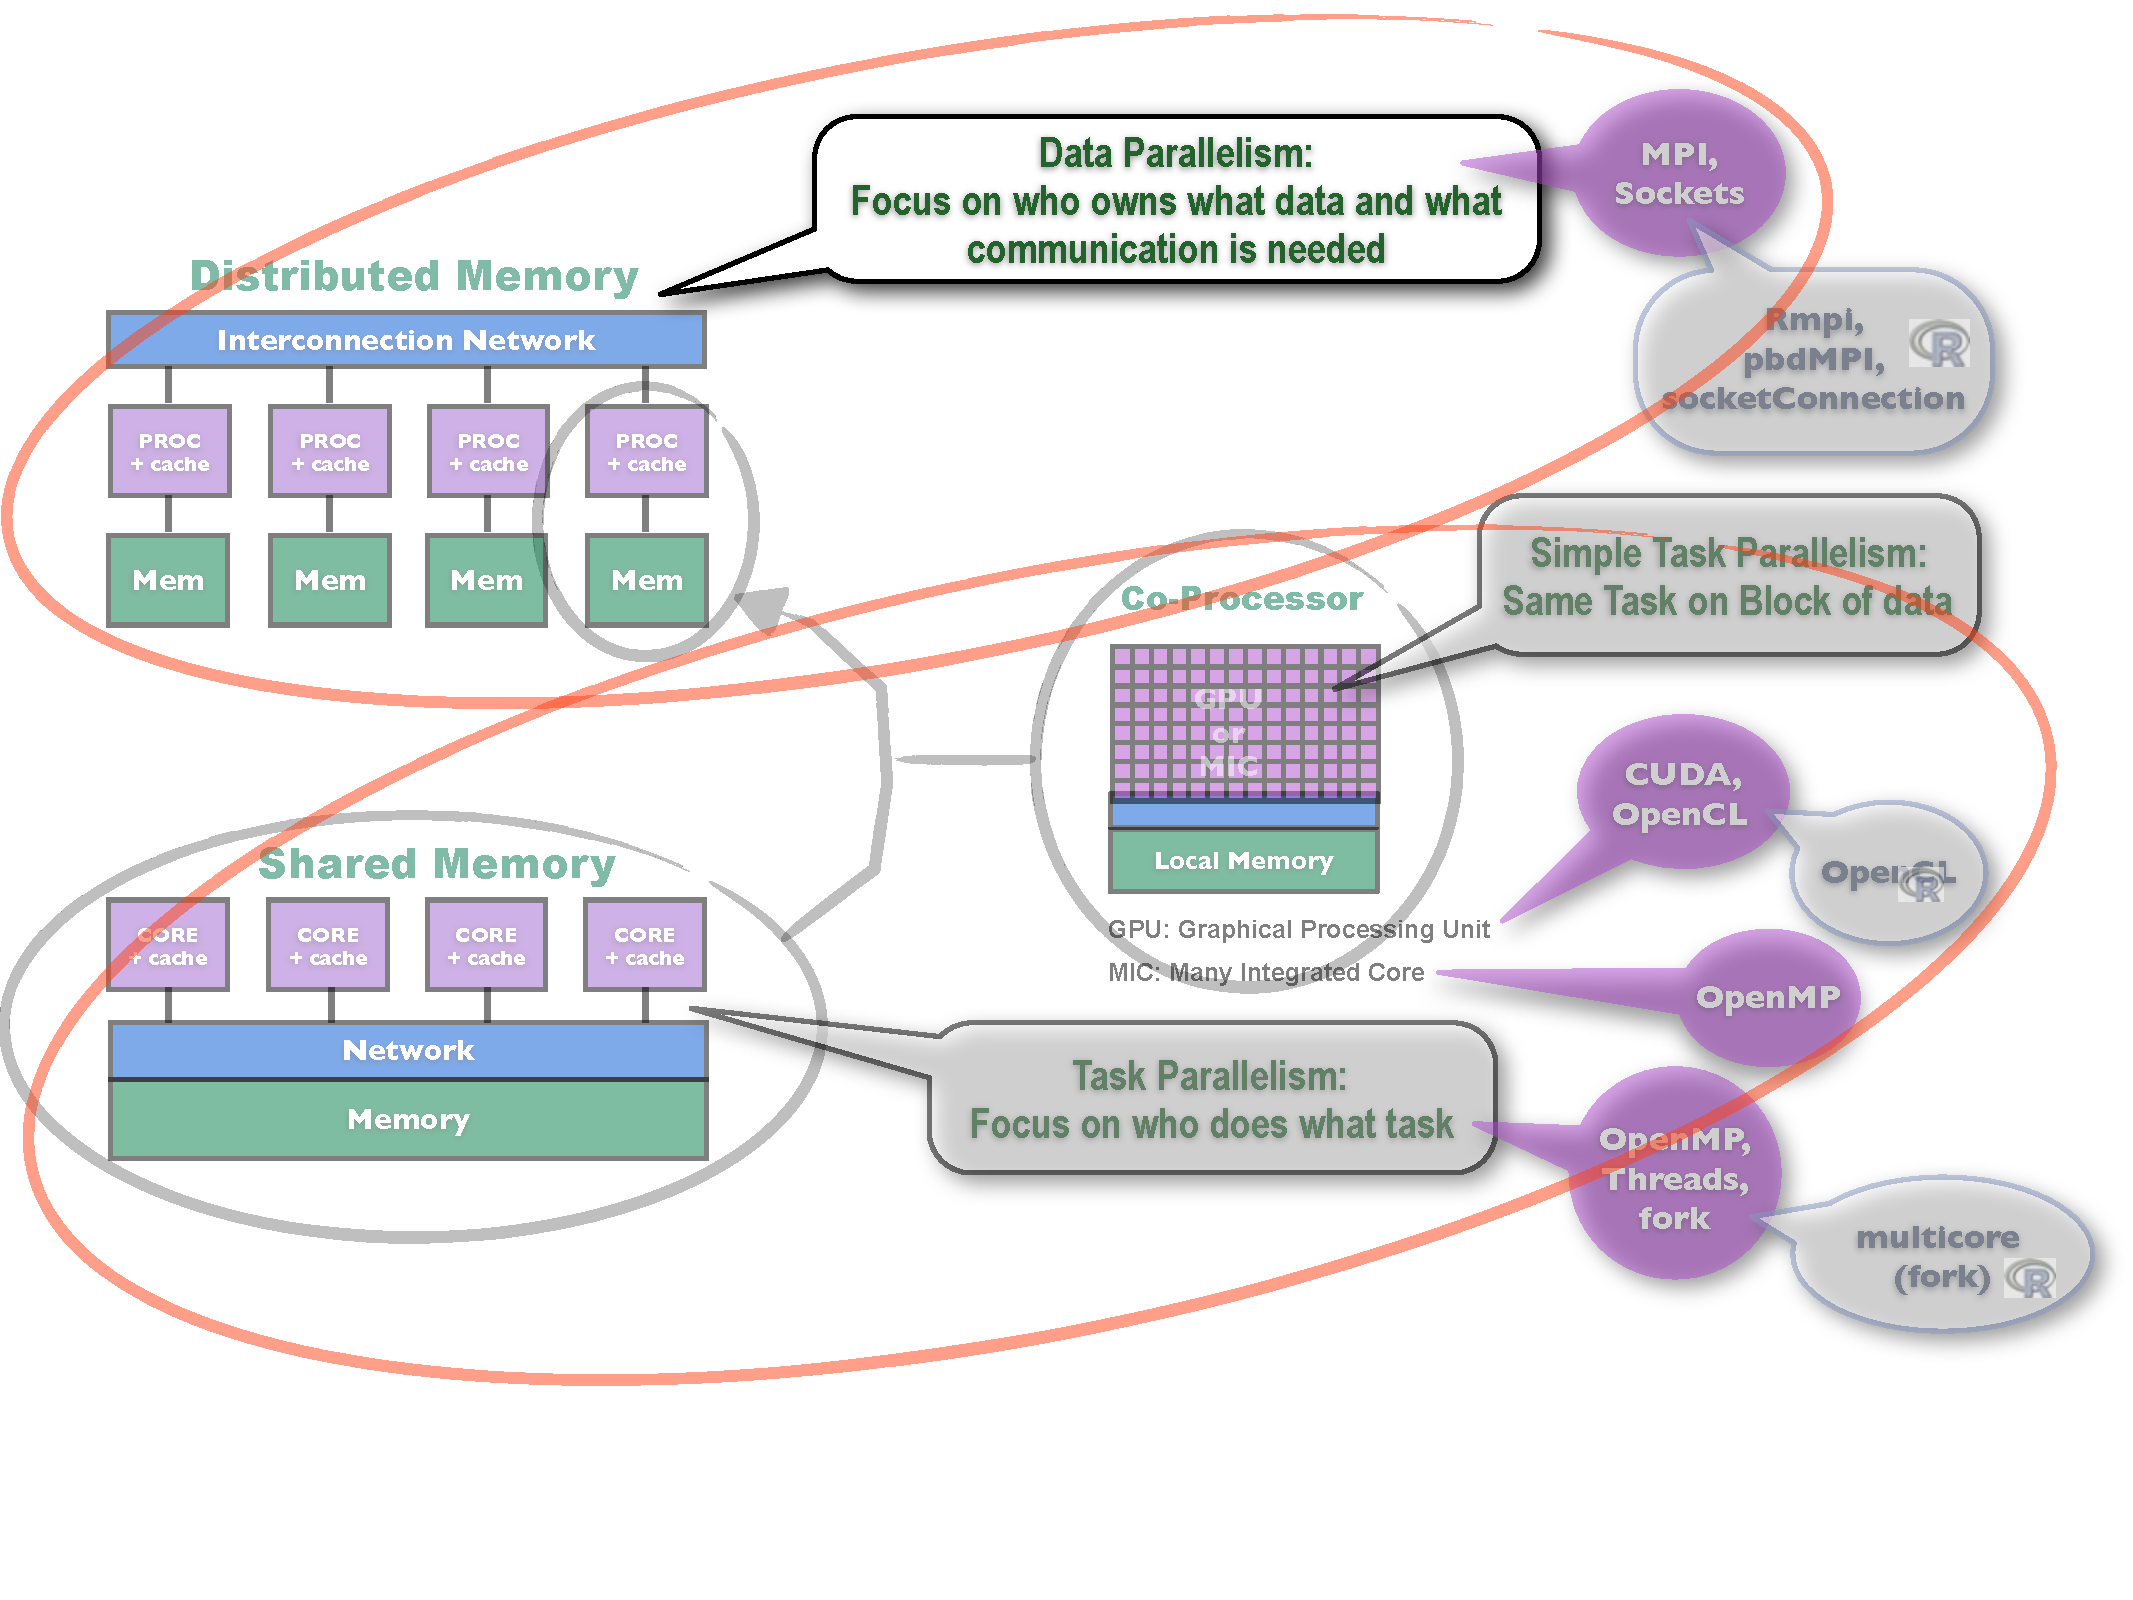
\includegraphics[width=0.95\textwidth]{../common/pics/ParallelHardware11.pdf}
\end{block}
\end{frame}


%%% Intro to parallelism
% \subsection{A Concise Introduction to Parallelism}

\begin{frame}
  \begin{block}{What is Parallelism?}\pause
  \begin{itemize}
    \item Doing more than one thing at a time.
    \item The simultaneous use of multiple compute resources to solve a 
computational problem.
  \end{itemize}
  \end{block}
\end{frame}

\begin{frame}
  \begin{block}{Parallelism}\pause
    \begin{center}
    \begin{minipage}{.46\textwidth}
    \begin{block}{\centering Serial Programming}
      \begin{center}
      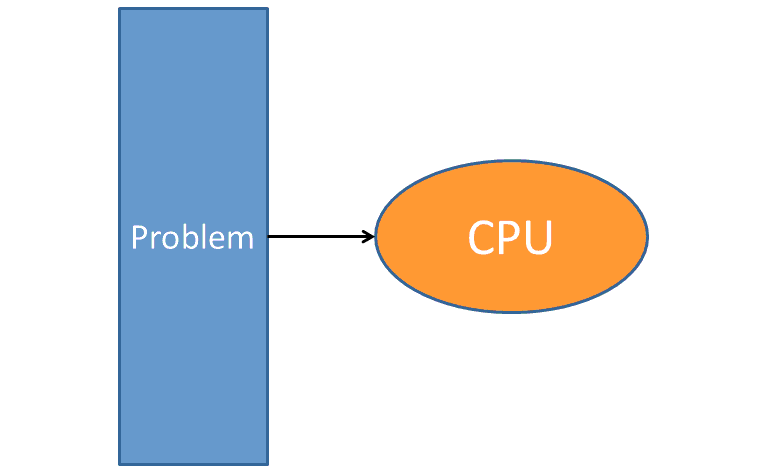
\includegraphics[width=.975\textwidth]{../common/pics/parallelism1}
      \end{center}
      \end{block}
    \end{minipage}
    \hspace{.15cm}
    \begin{minipage}{.46\textwidth}
    \begin{block}{\centering Parallel Programming}
      \begin{center}
      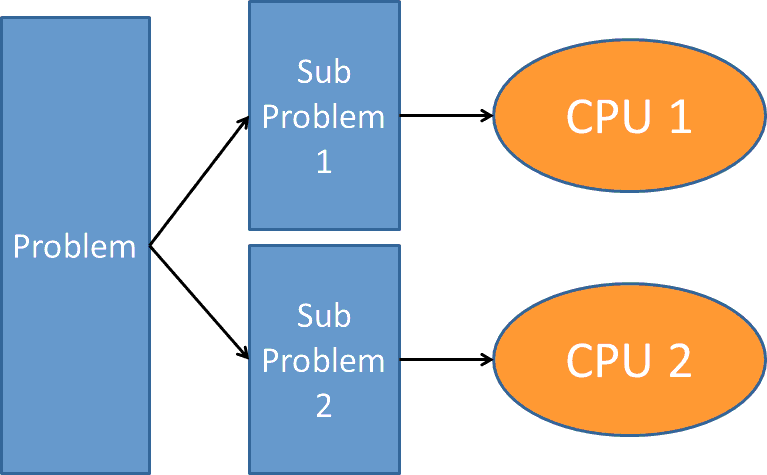
\includegraphics[width=.975\textwidth]{../common/pics/parallelism2}
      \end{center}
      \end{block}
    \end{minipage}
    \end{center}
  \end{block}
\end{frame}

\begin{frame}
  \begin{block}{Parallelism}\pause
    \begin{center}
    \begin{minipage}{.46\textwidth}
    \begin{block}{Serial Programming}
      \begin{center}
      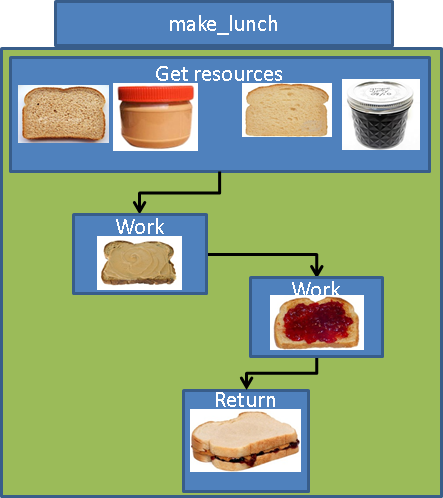
\includegraphics[width=.975\textwidth]{../common/pics/analogy_serial}
      \end{center}
      \end{block}
    \end{minipage}
    \hspace{.15cm}
    \begin{minipage}{.46\textwidth}
    \begin{block}{Parallel Programming}
      \begin{center}
      
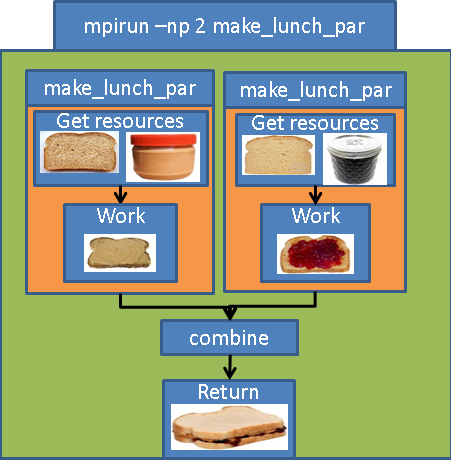
\includegraphics[height=5.45cm,width=.975\textwidth]{../common/pics/analogy_parallel}
      \end{center}
      \end{block}
    \end{minipage}
    \end{center}
  \end{block}
\end{frame}


\begin{frame}
  \begin{block}{Kinds of Parallelism}\pause
    \begin{itemize}[<+-|alert@+>]
      \item \emph{Data Parallelism}:  Data is distributed
      \item \emph{Task Parallelism}:  Tasks are distributed
  \end{itemize}
  (This is a gross oversimplification)
  \end{block}
\end{frame}


\begin{frame}
  \begin{block}{pbdR Paradigms:  Data Parallelism}
  Data parallelism:
  \begin{itemize}[<+-|alert@+>]
   \item No one processor/node owns all the data.
   \item Processors own local pieces of a (conceptually) larger, global object
  \end{itemize}
  
  Task parallelism:
  \begin{itemize}
    \item (Usually) Applying different tasks to the same data.
  \end{itemize}
  \end{block}
\end{frame}


\begin{frame}
  \begin{block}{Data vs Task Parallelism}\pause
    \begin{center}
    \begin{minipage}{.46\textwidth}
    \begin{block}{\centering Data Parallelism}
      \begin{center}
      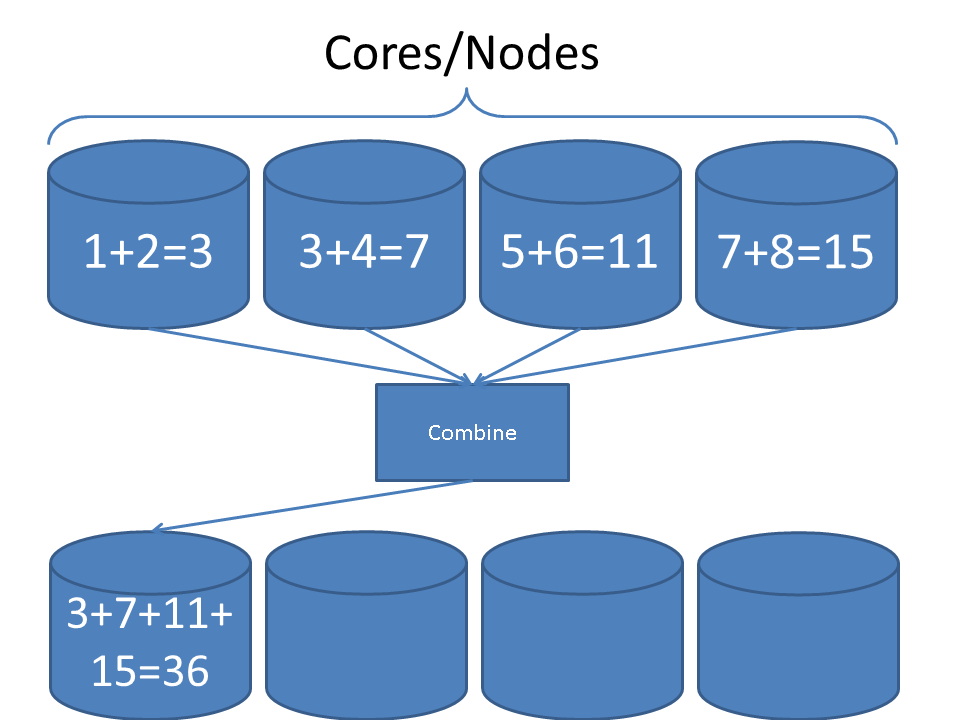
\includegraphics[width=.975\textwidth]{../common/pics/parallelism_data}
      \end{center}
      \end{block}
    \end{minipage}
    \hspace{.15cm}
    \begin{minipage}{.46\textwidth}
    \begin{block}{\centering Task Parallelism}
      \begin{center}
      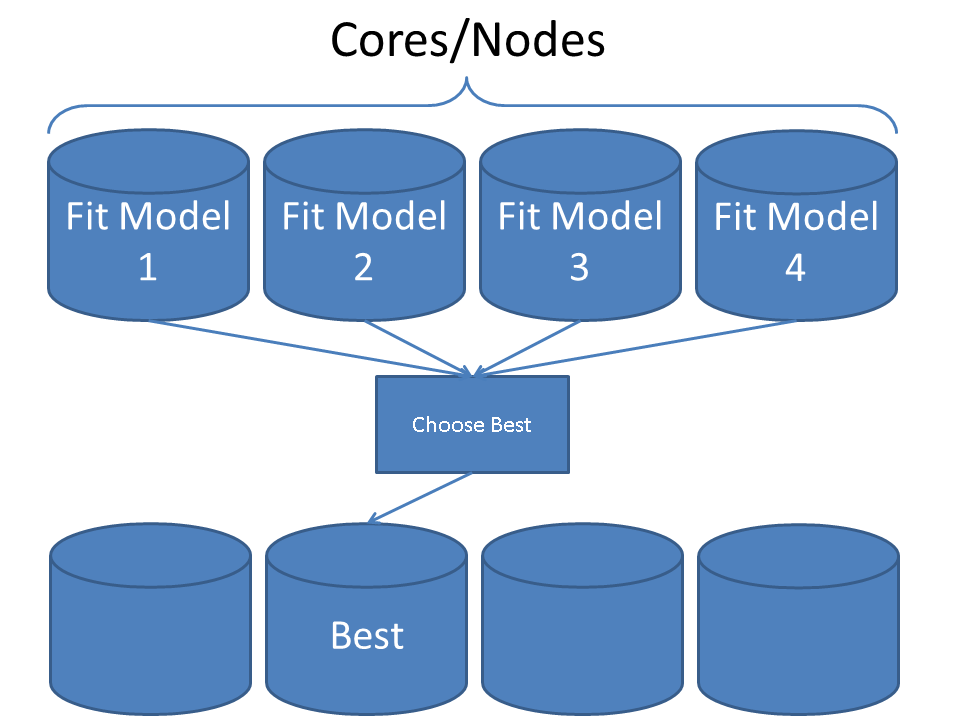
\includegraphics[width=.975\textwidth]{../common/pics/parallelism_task}
      \end{center}
      \end{block}
    \end{minipage}
    \end{center}
  \end{block}
\end{frame}




% \subsection{Common Terminology}


\begin{frame}
  \begin{block}{Parallel Programming Vocabulary:  Difficulty in Parallelism}
  \begin{enumerate}[<+-|alert@+>]
    \item \emph{Implicit parallelism}:  Parallel details hidden from user
    \item \emph{Explicit parallelism}:  Some assembly required\dots
    \item \emph{Embarrassingly Parallel}:  Also called \emph{loosely coupled}.  
Obvious how to make parallel; lots of independence in computations.
    \item \emph{Tightly Coupled}:  Opposite of embarrassingly parallel; lots of 
dependence in computations.
  \end{enumerate}  
  \end{block}
\end{frame}


\begin{frame}
  \begin{block}{Speedup}
  \begin{itemize}
    \item \emph{Wallclock Time}:  Time of the clock on the wall from start to 
finish
    \item \emph{Speedup}:  unitless measure of improvement; more is better.
  \begin{align*}
   S_{n_1, n_2} =  \frac{\text{Run time for } n_1 \text{ cores}}{\text{Run time 
for } n_2 \text{ cores}}
  \end{align*}
  \begin{itemize}
    \item   $n_1$ is often taken to be 1
    \item In this case, comparing parallel algorithm to serial algorithm
  \end{itemize}
  \end{itemize}
  \end{block}
\end{frame}


\begin{frame}
  \begin{block}{Speedup}
   \begin{center}
    \begin{minipage}{.475\textwidth}
    \begin{block}{Good Speedup}
      \centering
      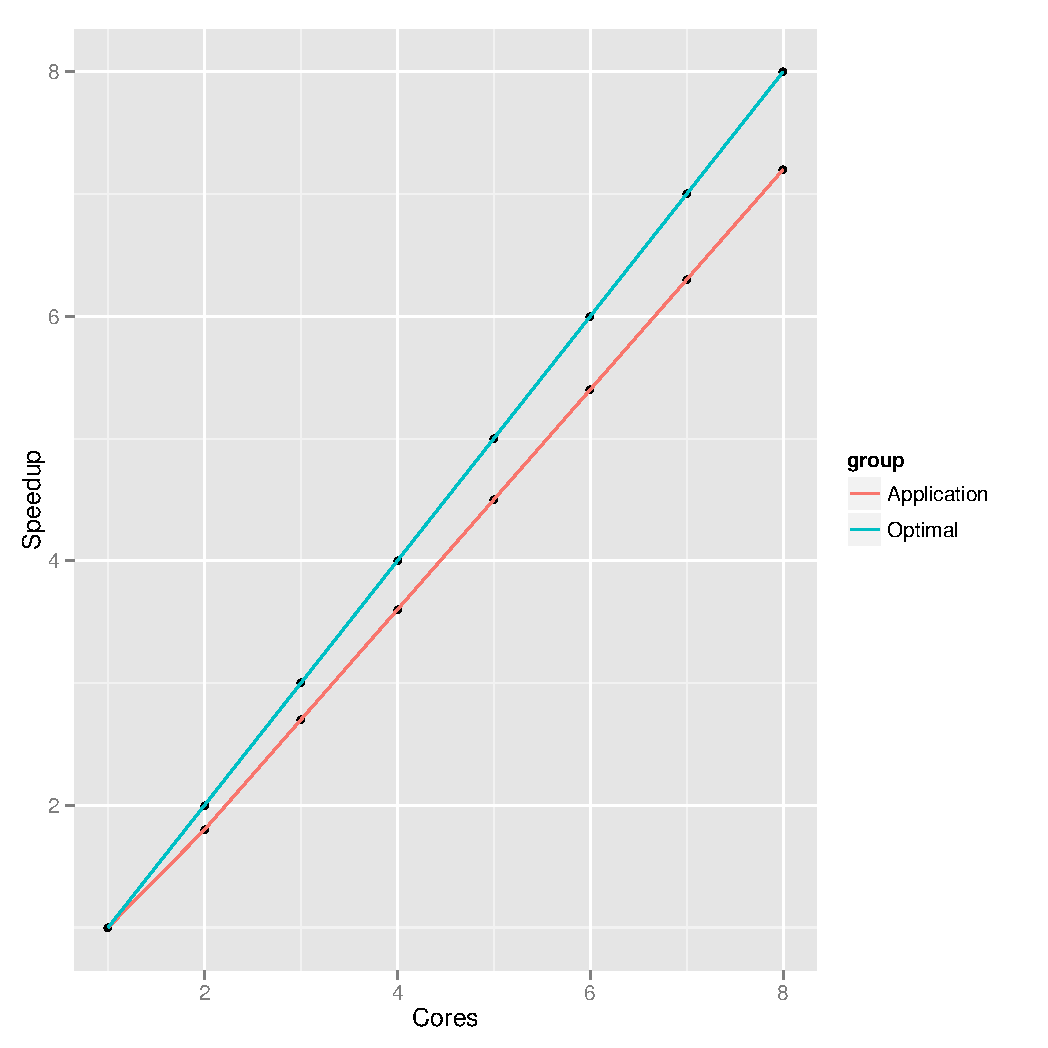
\includegraphics[width=.95\textwidth]{../common/pics/scale_good}
    \end{block}
    \end{minipage}
    \hspace{.1cm}
    \begin{minipage}{.475\textwidth}
    \begin{block}{Bad Speedup}
      \centering
      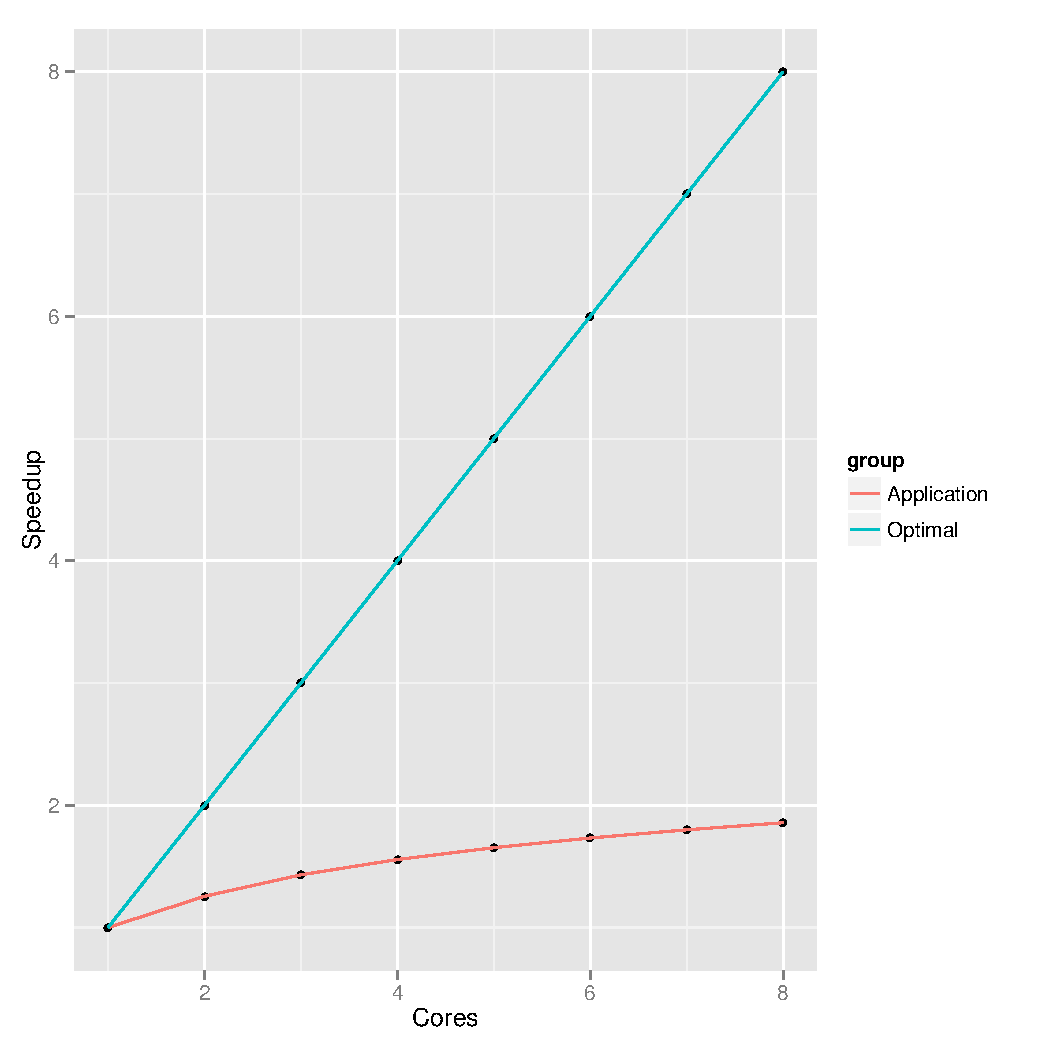
\includegraphics[width=.95\textwidth]{../common/pics/scale_bad}
    \end{block}
    \end{minipage}
    \end{center}
    \end{block}
\end{frame}


\begin{frame}
  \begin{block}{Shared and Distributed Memory Machines}
   \begin{center}
    \begin{minipage}{.475\textwidth}
    \begin{block}{Shared Memory}
     Direct access to read/change memory (one node) \vspace{.3cm} \ 
      \begin{center}
      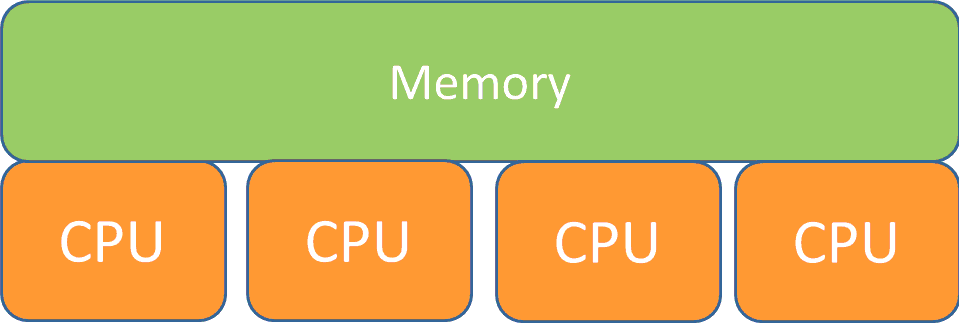
\includegraphics[width=.95\textwidth]{../common/pics/arch_shared}
      \end{center}
      \vspace{.3cm} \
    \end{block}
    \end{minipage}
    \hspace{.1cm}
    \begin{minipage}{.475\textwidth}
    \begin{block}{Distributed}
    No direct access to read/change memory (many nodes); requires communication
      \begin{center}
      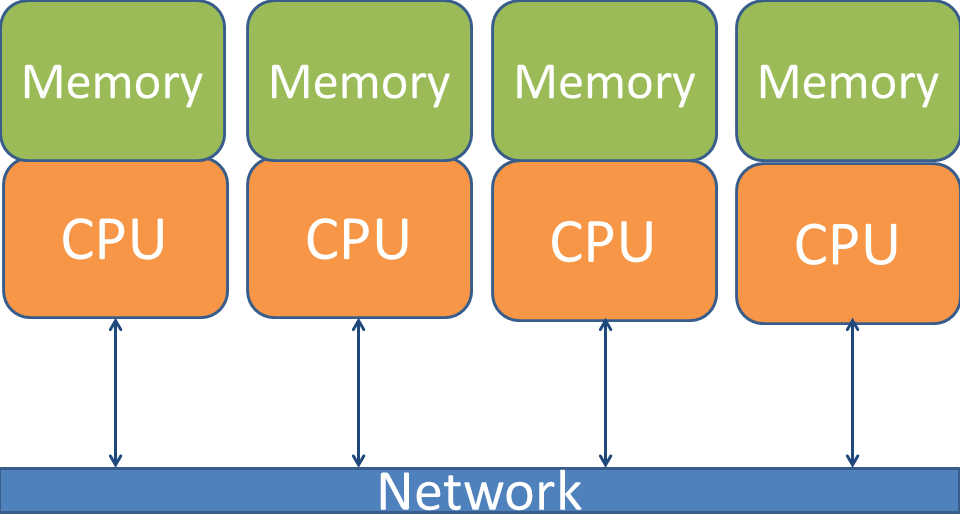
\includegraphics[width=.95\textwidth]{../common/pics/arch_distributed}
      \end{center}
    \end{block}
    \end{minipage}
    \end{center}
    \end{block}
\end{frame}


\begin{frame}
  \begin{block}{Shared and Distributed Memory Machines}
   \begin{center}
    \begin{minipage}[t]{.47\textwidth}
    \begin{block}{Shared Memory Machines}
    \begin{center}
    Thousands of cores\\[.2cm]
    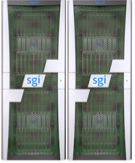
\includegraphics[scale=.65]{../common/pics/nautilus}\\
    {\tiny \emph{Nautilus}, University of Tennessee\\1024 cores \\4 TB RAM\\}
    \end{center}
    \end{block}
    \end{minipage}
    \hspace{.1cm}
    \begin{minipage}[t]{.47\textwidth}
    \begin{block}{Distributed Memory Machines}
    \begin{center}
    Hundreds of thousands of cores\\[.2cm]
    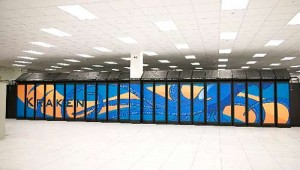
\includegraphics[width=.95\textwidth]{../common/pics/kraken}\\
    {\tiny \emph{Kraken}, University of Tennessee\\ 112,896 cores \\147 TB 
RAM\\}
    \end{center}
    \end{block}
    \end{minipage}
    \end{center}
    \end{block}
\end{frame}




\subsection{R and Parallelism}


\begin{frame}
%  \addtocounter{framenumber}{-1}
  \begin{block}{R and Parallelism}\pause
  What about R?
  \end{block}
\end{frame}

\begin{frame}
%  \addtocounter{framenumber}{-1}
  \begin{block}{Problems with Serial R}\pause
  \begin{enumerate}[<+-|alert@+>]
    \item Slow.
    \item If you don't know what you're doing, it's \emph{really} slow.
    \item Performance improvements usually for small machines.
    \item Very ram intensive.
  \end{enumerate}
  \end{block}
\end{frame}


\begin{frame}
  \begin{block}{Why We Need Parallelism}\pause
    \begin{enumerate}[<+-|alert@+>]
      \item Saves compute time.
      \item Data size is skyrocketing.
      \item Necessary for many problems.
      \item Its necessity is coming.
      \item \emph{It's really cool.}
  \end{enumerate}
  \end{block}
\end{frame}

\begin{frame}
  \begin{block}{Recall: Parallel R Packages}
   \begin{center}
    \begin{minipage}{.45\textwidth}
    \begin{block}{Shared Memory}
      \begin{enumerate}[<+-|alert@+>]
        \item \pkg{foreach}
        \item \pkg{parallel}
        \item \pkg{snow}
        \item \pkg{multicore}
      \end{enumerate}
    \end{block}
    \end{minipage}
    \hspace{.2cm}
    \begin{minipage}{.45\textwidth}
    \begin{block}{Distributed}
      \begin{enumerate}[<+-|alert@+>]
        \item \pkg{Rmpi}
        \item R+Hadoop
        \item \pkg{pbdR}
      \end{enumerate}
    \end{block}
    \end{minipage}
    \end{center}
    (and others\dots)
    \end{block}
\end{frame}



\begin{frame}[shrink]
  \begin{block}{R and Parallelism}
    The solution to many of R's problems is parallelism.  However \dots\vspace{-.4cm}
   \begin{center}
    \begin{minipage}[t]{.95\textwidth}
    \begin{block}{\centering What we have}
      \begin{enumerate}[<+-|alert@+>]
        \item Mostly serial.
        \item Mostly not distributed
        \item Data parallelism mostly explicit
      \end{enumerate}
    \end{block}
    \end{minipage}
    \\\pause
    \begin{minipage}[t]{.95\textwidth}
    \begin{block}{\centering What we want}
      \begin{enumerate}[<+-|alert@+>]
        \item Mostly parallel.
        \item Mostly distributed.
        \item Mostly implicit.
      \end{enumerate}
    \end{block}
    \end{minipage}
    \end{center}
    \end{block}
\end{frame}



\begin{frame}
  \begin{block}{R and Parallelism}
    Likewise, the HPC community is looking for high-level languages for data\dots
    \end{block}
\end{frame}


\section{pbdR}
\makesubcontentsslides

\subsection{The pbdR Project}
\makesubcontentsslidessec

\begin{frame}{\pbdR Interfaces to Libraries: Sustainable Path}
  \vspace{-1ex}
  \centering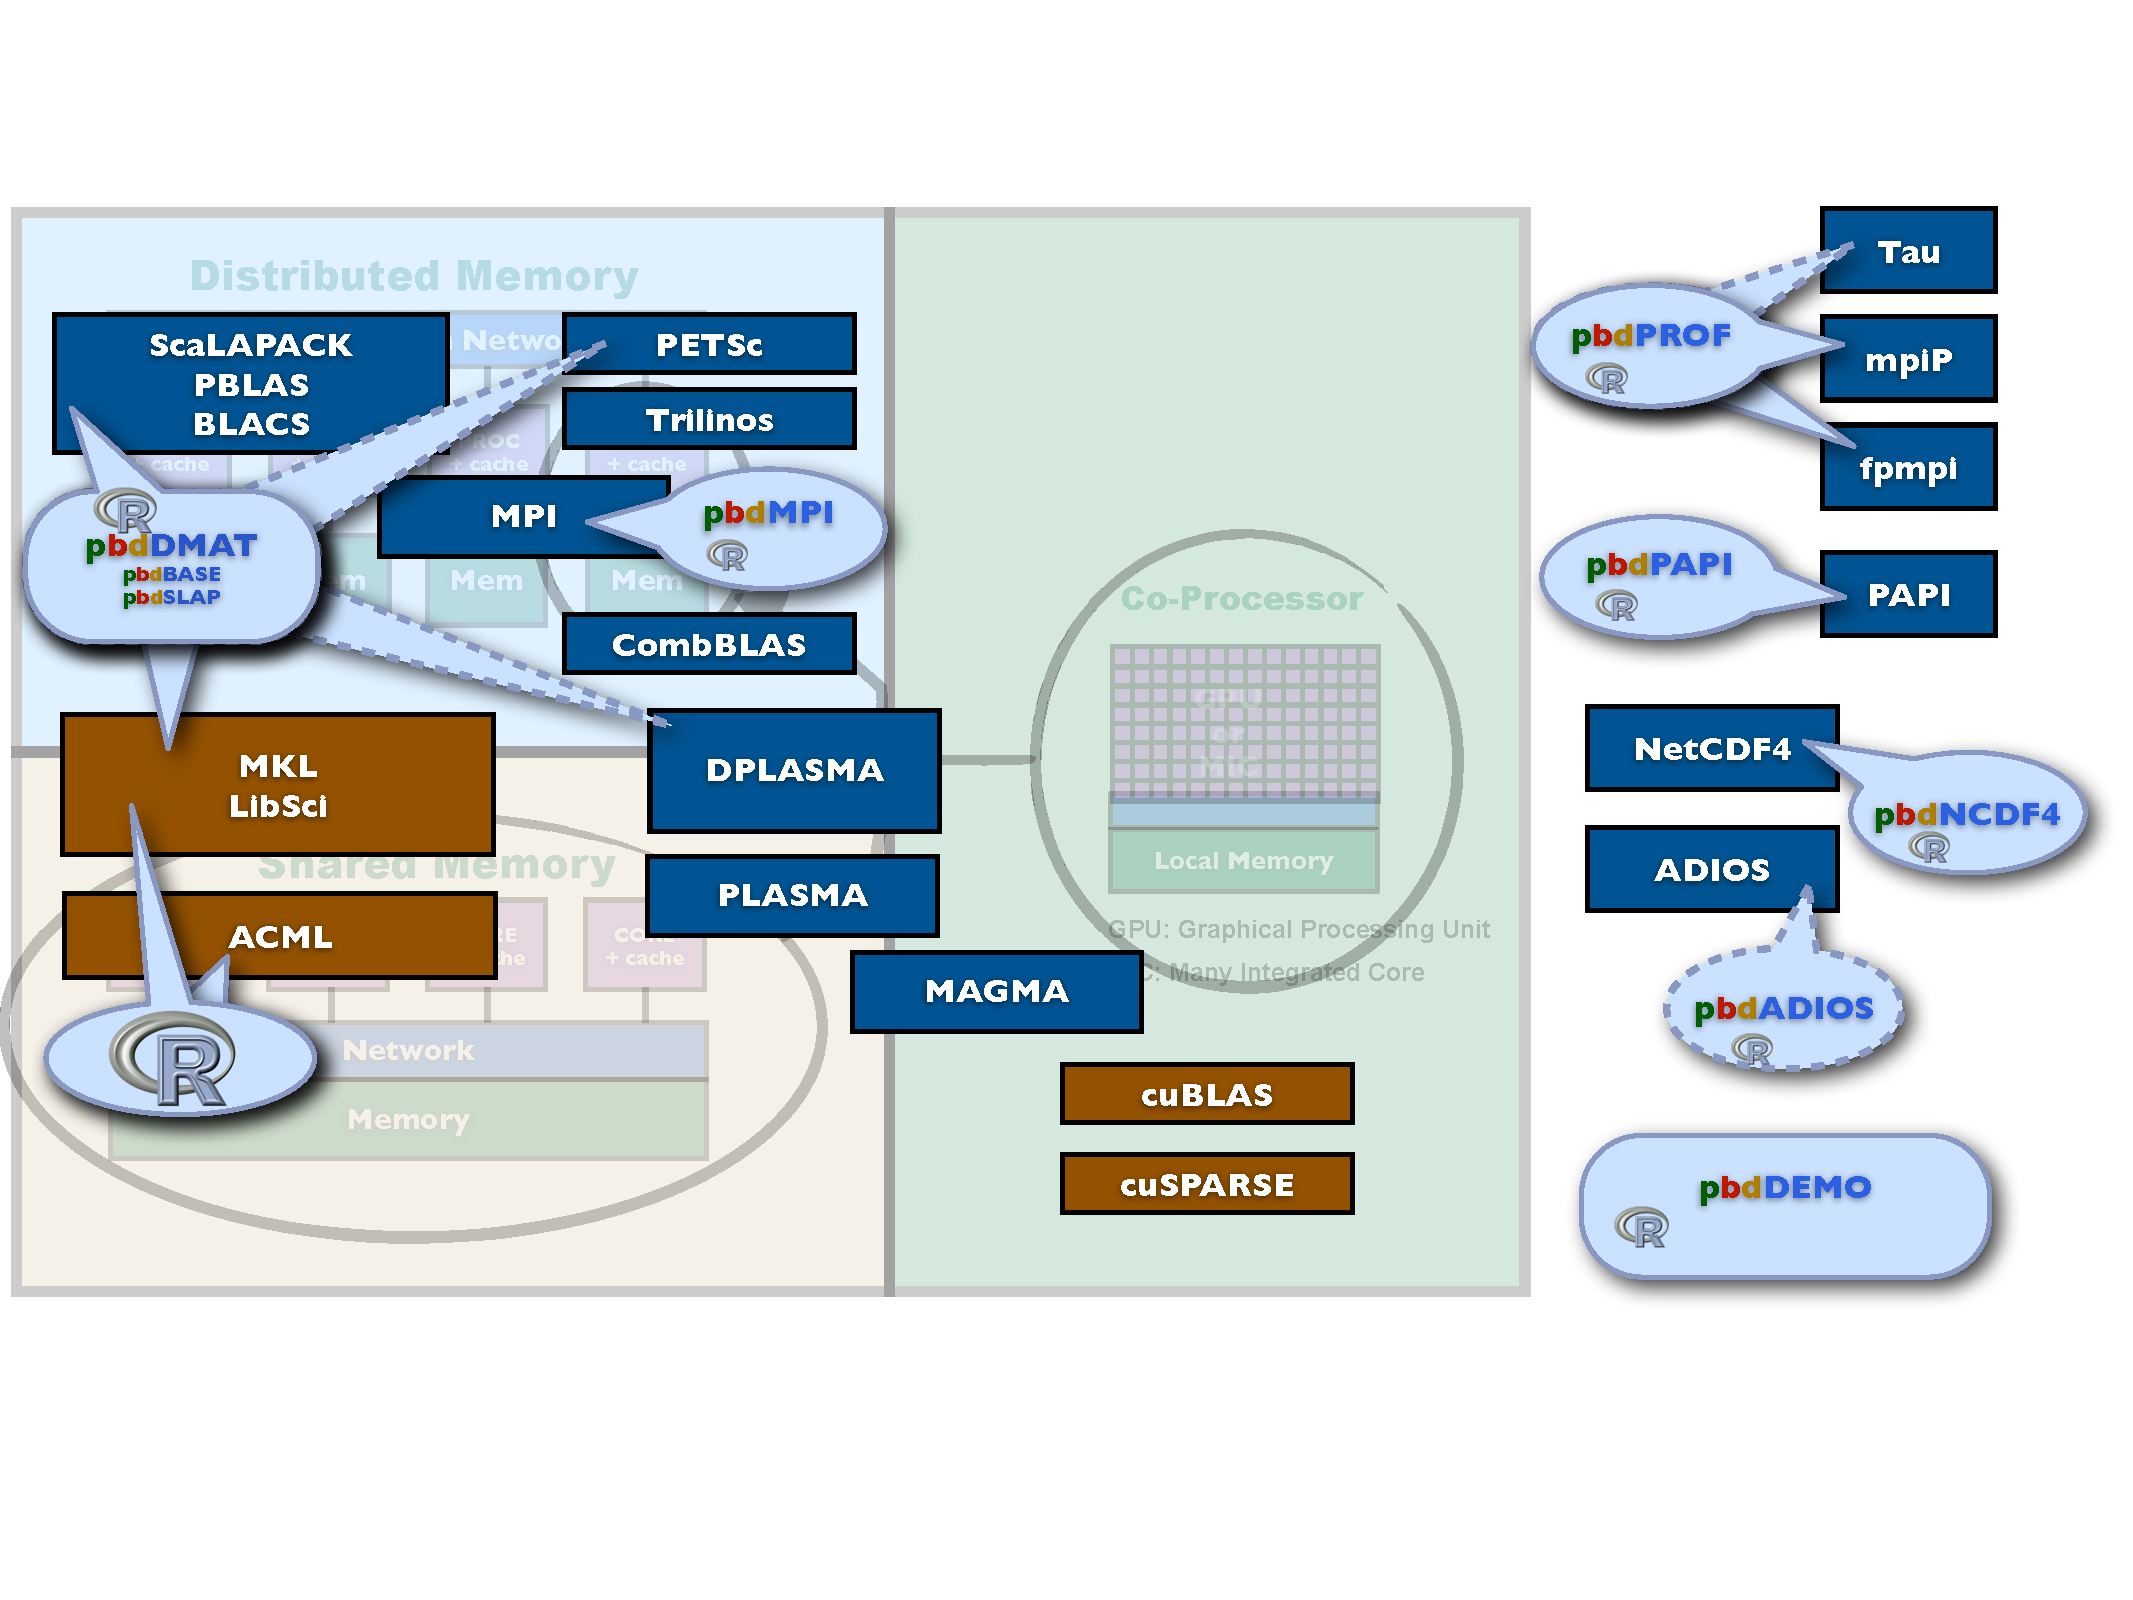
\includegraphics[trim=0cm 5cm 0cm 3cm,clip=true,width=0.85\textwidth]
  {../common/pics/hardware/ParallelHardware27.pdf}
  \scriptsize
  \begin{block}{Why use HPC libraries?}
    \begin{itemize}[<+-|alert@+>]
    \item The HPC community is 30 years beyond ``embarrassingly parallel.''
    \item \emph{They're tested.} \emph{They're
        fast.}  \emph{They're scalable.}
    \item Many science communities are invested in their API.
    \item Data analysis uses much of the same math as simulation science.
    \end{itemize}
  \end{block}
\end{frame}

\subsection{pbdMPI}
\makesubcontentsslidessec

\begin{frame}
  \begin{block}{pbdMPI: a High Level Interface to MPI}
    \begin{itemize}
    \item API is simplified: defaults in control objects.
    \item S4 methods: extensible to complex \R objects.
    \item Additional error checking
    \item Array and matrix methods without serialization: faster than
      \pkg{Rmpi}.
    \end{itemize}
    \begin{center}
      \vspace{0.2cm}\scriptsize
      \begin{tabular}{ll} \hline\hline
        \pkg{pbdMPI} (S4) & \pkg{Rmpi}                \\ \hline
        \code{\color{blue}allreduce}    & \code{mpi.allreduce}      \\
        \code{\color{blue}allgather}    & \code{mpi.allgather},
        \code{mpi.allgatherv},
        \code{mpi.allgather.Robj} \\
        \code{bcast}        & \code{mpi.bcast},
        \code{mpi.bcast.Robj}     \\
        \code{gather}       & \code{mpi.gather},
        \code{mpi.gatherv},
        \code{mpi.gather.Robj}    \\
        \code{recv}         & \code{mpi.recv},
        \code{mpi.recv.Robj}      \\
        \code{reduce}       & \code{mpi.reduce}         \\
        \code{scatter}      & \code{mpi.scatter},
        \code{mpi.scatterv},
        \code{mpi.scatter.Robj}   \\
        \code{send}         & \code{mpi.send},
        \code{mpi.send.Robj}      \\ \hline \hline
      \end{tabular}
    \end{center}
  \end{block}
\end{frame}

\begin{frame}[fragile]
  \begin{block}{Integer?\qquad Not always obvious in R.}
    \vspace{-.2cm}
    \begin{lstlisting}
> is.integer(1)
[1] FALSE
> is.integer(2)
[1] FALSE
> is.integer(1:2)
[1] TRUE
    \end{lstlisting}
  \end{block}
  \begin{block}{Often it's best to let the machine figure it out}\pause
    \begin{minipage}[t]{.475\textwidth}
      \begin{lstlisting}[title=Rmpi]
# int
mpi.allreduce(x, type=1)
# double
mpi.allreduce(x, type=2)
      \end{lstlisting}
    \end{minipage}
    \hfill
    \begin{minipage}[t]{.475\textwidth}
      \begin{lstlisting}[title=pbdMPI]
allreduce(x)
      \end{lstlisting}
      % \vspace{1em}
      % \hspace{1em}{\small S4. Batch only! (No spawning)}
    \end{minipage}
  \end{block}
\end{frame}



% \begin{frame}[fragile,shrink]
%   \begin{block}{Embarrassingly Parallel Computation}\pause
%     \vspace{-1ex}
%     \begin{minipage}[t]{.45\textwidth}
%       \begin{lstlisting}[title=EPforeach.R "asking for parallel",basicstyle=\tiny]
% library(doMPI, quiet=TRUE)
% cl <- startMPIcluster()
% registerDoMPI(cl)

% n <- 10
% myIn <- vector("list", n)

% myFun <- function(x) {
%   s <- sum(rnorm(10000))
%   rank <- mpi.comm.rank(comm=0)
%   return(paste(s, "from", rank))
% }

% results <- foreach(i = 1:n) %dopar% {
%   out <- myFun(myIn[[i]])
% }

% print(results)

% closeCluster(cl)
% mpi.quit()
%       \end{lstlisting}
%     \end{minipage}
%     \hfill
%     \begin{minipage}[t]{.5\textwidth}
%       \begin{lstlisting}[title=EPpbdR.R "thinking parallel",basicstyle=\tiny]
% library(pbdMPI, quiet=TRUE)
% init()

% myChunk <- get.jid(n <- 10)
% myIn <- vector("list", length(myChunk))
% myOut <- vector("list", length(myChunk))

% myFun = function(x) {
%   s <- sum(rnorm(10000))
%   rank <- comm.rank()
%   return(paste(s, "from", rank))
% }

% for(i in 1:length(myChunk)) {
%   myOut[[i]] <- myFun(myIn[[i]])
% }
% results <- gather(myOut)

% comm.print(results)
% finalize()
%       \end{lstlisting}
%     \end{minipage}
%   \end{block}
% \end{frame}


\begin{frame}[fragile]{SPMD Runs Many Copies of One Code}
  \begin{exampleblock}{SPMD Hello World: a ``map-reduce'' to all}
    \vspace{-1.5ex}
    \centering
    \begin{lstlisting}[title=map-reduce.r]
library(pbdMPI, quiet = TRUE)
init()

## Your "Map" code
n <- comm.rank() + 1

## Now "Reduce" but give the result to all
all_sum <- allreduce(n) # Sum is default

text <- paste("Hello: n is", n, "sum is", all_sum )
comm.print(text, all.rank=TRUE)

finalize()
    \end{lstlisting}
    \vspace{-4.5ex}
    \begin{columns}[t,onlytextwidth]
      \begin{column}{0.54\textwidth}
        \begin{lstlisting}[backgroundcolor=\color{white},keywordstyle=\color{black},
title=Execute this batch script via:]
mpirun -np 2 Rscript map-reduce.r
        \end{lstlisting}
      \end{column}
      \hfill
      \begin{column}{0.46\textwidth}
        \begin{lstlisting}[title=Output:]
COMM.RANK = 0
[1] "Hello: n is 1 sum is 3"
COMM.RANK = 1
[1] "Hello: n is 2 sum is 3"
        \end{lstlisting}
      \end{column}
    \end{columns}
  \end{exampleblock}
\end{frame}

\subsection{pbdDMAT}
\makesubcontentsslidessec

\begin{frame}{Dense Matrix and Vector Operations}
  \begin{block}{A matrix is mapped to a processor grid shape}
    \begin{table}[ht]
      \centering
      % \begin{subfigure}[b]{0.23\textwidth}
      %   \centering
      %   $\left[\begin{tabular}{l}
      %       0 \\ 1 \\ 2 \\ 3 \\ 4 \\ 5
      %     \end{tabular}\right]^T$
      %   \caption{$1\times 6$}
      % \end{subfigure}
      \begin{subfigure}[b]{0.23\textwidth}
        \centering
        $\left[\begin{tabular}{llllll}
            0 & 1 & 2 & 3 & 4 & 5
          \end{tabular}\right]$
        \vspace{1.5cm}
        \caption{$1\times 6$}
      \end{subfigure}%\hspace{-1cm}
      \begin{subfigure}[b]{0.23\textwidth}
        \centering
        $\left[\begin{tabular}{lll}
            0 & 1 & 2\\
            3 & 4 & 5
          \end{tabular}\right]$
        \caption{$2\times 3$}
      \end{subfigure}%
      \begin{subfigure}[b]{0.23\textwidth}
        \centering
        $\left[\begin{tabular}{ll}
            0 & 1 \\
            2 & 3\\
            4 & 5
          \end{tabular}\right]$
        \caption{$3\times 2$}
      \end{subfigure}
      \begin{subfigure}[b]{0.23\textwidth}
        \centering
        $\left[\begin{tabular}{l}
            0 \\ 1 \\ 2 \\ 3 \\ 4 \\ 5
          \end{tabular}\right]$
        \caption{$6\times 1$}
      \end{subfigure}
      \caption{Processor Grid Shapes with 6 Processors}\label{fig:gridshapes}
    \end{table}
  \end{block}
\end{frame}

\begin{frame}[shrink]
\begin{exampleblock}{2$\times$3 block-cyclic grid on 6 processors:
    Global view ``ddmatrix'' class}
\begin{align*}
x &= \left[
      \begin{array}{ll|ll|ll|ll|l}
      \color{g11}x_{11} & \color{g11}x_{12} & \color{g12}x_{13} & \color{g12}x_{14} & \color{g13}x_{15} & \color{g13}x_{16} & \color{g11}x_{17} & \color{g11}x_{18} & \color{g12}x_{19}\\
      \color{g11}x_{21} & \color{g11}x_{22} & \color{g12}x_{23} & \color{g12}x_{24} & \color{g13}x_{25} & \color{g13}x_{26} & \color{g11}x_{27} & \color{g11}x_{28} & \color{g12}x_{29}\\\hline
      \color{g21}x_{31} & \color{g21}x_{32} & \color{g22}x_{33} & \color{g22}x_{34} & \color{g23}x_{35} & \color{g23}x_{36} & \color{g21}x_{37} & \color{g21}x_{38} & \color{g22}x_{39}\\
      \color{g21}x_{41} & \color{g21}x_{42} & \color{g22}x_{43} & \color{g22}x_{44} & \color{g23}x_{45} & \color{g23}x_{46} & \color{g21}x_{47} & \color{g21}x_{48} & \color{g22}x_{49}\\\hline
      \color{g11}x_{51} & \color{g11}x_{52} & \color{g12}x_{53} & \color{g12}x_{54} & \color{g13}x_{55} & \color{g13}x_{56} & \color{g11}x_{57} & \color{g11}x_{58} & \color{g12}x_{59}\\
      \color{g11}x_{61} & \color{g11}x_{62} & \color{g12}x_{63} & \color{g12}x_{64} & \color{g13}x_{65} & \color{g13}x_{66} & \color{g11}x_{67} & \color{g11}x_{68} & \color{g12}x_{69}\\\hline
      \color{g21}x_{71} & \color{g21}x_{72} & \color{g22}x_{73} & \color{g22}x_{74} & \color{g23}x_{75} & \color{g23}x_{76} & \color{g21}x_{77} & \color{g21}x_{78} & \color{g22}x_{79}\\
      \color{g21}x_{81} & \color{g21}x_{82} & \color{g22}x_{83} & \color{g22}x_{84} & \color{g23}x_{85} & \color{g23}x_{86} & \color{g21}x_{87} & \color{g21}x_{88} & \color{g22}x_{89}\\\hline
      \color{g11}x_{91} & \color{g11}x_{92} & \color{g12}x_{93} & \color{g12}x_{94} & \color{g13}x_{95} & \color{g13}x_{96} & \color{g11}x_{97} & \color{g11}x_{98} & \color{g12}x_{99}\\
      \end{array}
\right]_{9\times 9}
\end{align*}
\begin{align*}
\text{Processor grid = }\left|
      \begin{array}{lll}
      \color{g11}0 & \color{g12}1 & \color{g13}2\\
      \color{g21}3 & \color{g22}4 & \color{g23}5
      \end{array}
\right| &=
\left|
      \begin{tabular}{lll}
      \color{g11}(0,0) & \color{g12}(0,1) & \color{g13}(0,2)\\
      \color{g21}(1,0) & \color{g22}(1,1) & \color{g23}(1,2)
      \end{tabular}
\right|
\end{align*}
\end{exampleblock}
\end{frame}


\begin{frame}[shrink]
\begin{exampleblock}{2$\times$3 block-cyclic grid on 6 processors:
    Local view ``ddmatrix'' class}
\begin{align*}
\left[
      \begin{array}{ll|ll}
      \color{g11}x_{11} & \color{g11}x_{12} & \color{g11}x_{17} & \color{g11}x_{18}\\
      \color{g11}x_{21} & \color{g11}x_{22} & \color{g11}x_{27} & \color{g11}x_{28}\\\hline
      \color{g11}x_{51} & \color{g11}x_{52} & \color{g11}x_{57} & \color{g11}x_{58}\\
      \color{g11}x_{61} & \color{g11}x_{62} & \color{g11}x_{67} & \color{g11}x_{68}\\\hline
      \color{g11}x_{91} & \color{g11}x_{92} & \color{g11}x_{97} & \color{g11}x_{98}\\
      \end{array}
\right]_{5\times 4}
\left[
      \begin{array}{ll|l}
      \color{g12}x_{13} & \color{g12}x_{14} & \color{g12}x_{19}\\
      \color{g12}x_{23} & \color{g12}x_{24} & \color{g12}x_{29}\\\hline
      \color{g12}x_{53} & \color{g12}x_{54} & \color{g12}x_{59}\\
      \color{g12}x_{63} & \color{g12}x_{64} & \color{g12}x_{69}\\\hline
      \color{g12}x_{93} & \color{g12}x_{94} & \color{g12}x_{99}\\
      \end{array}
\right]_{5\times 3}
\left[
      \begin{array}{ll}
      \color{g13}x_{15} & \color{g13}x_{16}\\
      \color{g13}x_{25} & \color{g13}x_{26}\\\hline
      \color{g13}x_{55} & \color{g13}x_{56}\\
      \color{g13}x_{65} & \color{g13}x_{66}\\\hline
      \color{g13}x_{95} & \color{g13}x_{96}\\
      \end{array}
\right]_{5\times 2}
\\
\left[
      \begin{array}{ll|ll}
      \color{g21}x_{31} & \color{g21}x_{32} & \color{g21}x_{37} & \color{g21}x_{38}\\
      \color{g21}x_{41} & \color{g21}x_{42} & \color{g21}x_{47} & \color{g21}x_{48}\\\hline
      \color{g21}x_{71} & \color{g21}x_{72} & \color{g21}x_{77} & \color{g21}x_{78}\\
      \color{g21}x_{81} & \color{g21}x_{82} & \color{g21}x_{87} & \color{g21}x_{88}\\
      \end{array}
\right]_{4\times 4}
\left[
      \begin{array}{ll|l}
      \color{g22}x_{33} & \color{g22}x_{34} & \color{g22}x_{39}\\
      \color{g22}x_{43} & \color{g22}x_{44} & \color{g22}x_{49}\\\hline
      \color{g22}x_{73} & \color{g22}x_{74} & \color{g22}x_{79}\\
      \color{g22}x_{83} & \color{g22}x_{84} & \color{g22}x_{89}\\
      \end{array}
\right]_{4\times 3}
\left[
      \begin{array}{ll}
      \color{g23}x_{35} & \color{g23}x_{36} \\
      \color{g23}x_{45} & \color{g23}x_{46} \\\hline
      \color{g23}x_{75} & \color{g23}x_{76} \\
      \color{g23}x_{85} & \color{g23}x_{86} \\
      \end{array}
\right]_{4\times 2}
\end{align*}
\begin{align*}
\text{Processor grid = }\left|
      \begin{array}{lll}
      \color{g11}0 & \color{g12}1 & \color{g13}2\\
      \color{g21}3 & \color{g22}4 & \color{g23}5
      \end{array}
\right| &=
\left|
      \begin{tabular}{lll}
      \color{g11}(0,0) & \color{g12}(0,1) & \color{g13}(0,2)\\
      \color{g21}(1,0) & \color{g22}(1,1) & \color{g23}(1,2)
      \end{tabular}
\right|
\end{align*}
\end{exampleblock}
\end{frame}

\begin{frame}[fragile]
  \begin{block}{\pbdR\ No change in syntax. \hfill Data redistribution functions.}
\vspace{-2ex}
  \begin{lstlisting}
x <- x[-1, 2:5]
x <- log(abs(x) + 1)
x.pca <- prcomp(x)
xtx <- t(x) %*% x
ans <- svd(solve(xtx))
  \end{lstlisting}
\vspace{-1ex}
  \begin{center}
  \emph{The above (and over 100 other functions) runs on 1 core with R \\
    or 10,000 cores with \pbdR ddmatrix class}
  \end{center}
\vspace{-2ex}
\begin{lstlisting}
> showClass("ddmatrix")
Class "ddmatrix" [package "pbdDMAT"]
Slots:
Name:     Data     dim    ldim   bldim   ICTXT
Class:  matrix numeric numeric numeric numeric
\end{lstlisting}
\vspace{-2ex}
\begin{lstlisting}
> x <- as.rowblock(x)
> x <- as.colblock(x)
> x <- redistribute(x, bldim=c(8, 8), ICTXT = 0)
\end{lstlisting}
  \end{block}
\end{frame}

\subsection{RandSVD}
\makesubcontentsslidessec


\begin{frame}[fragile]
\fontsize{8pt}{10}\selectfont
\begin{block}{Randomized truncated SVD\footnotemark}
  \begin{minipage}{.56\textwidth}
    \begin{center}
      \includegraphics[height=.41\textheight]{../common/pics/randsvd/randSVDalg}
      \\
      \includegraphics[height=.26\textheight]{../common/pics/randsvd/randSVDalg4_4}
    \end{center}
  \end{minipage}
%   \hspace{.01cm}
  \begin{minipage}{0.43\textwidth}
\begin{lstlisting}[title=Serial 
R,basicstyle=\tiny,backgroundcolor=\color{grayish} 
,numberstyle=\tiny\color{black},keywordstyle=\color{black},commentstyle=\color{ 
dkgreen},stringstyle=\color{black},escapeinside={(*@}{@*)}]
randSVD <- function(A, k, q=3)
  {
    ## Stage A
    Omega <- (*@ matrix(rnorm(n*2*k),@*)
      (*@ nrow=n, ncol=2*k) @*)
    Y <- A %*% Omega
    Q <- qr.Q(qr(Y))
    At <- t(A)
    for(i in 1:q)
      {
        Y <- At %*% Q
        Q <- qr.Q(qr(Y))
        Y <- A %*% Q
        Q <- qr.Q(qr(Y))
      }
    
    ## Stage B
    B <- t(Q) %*% A
    U <- La.svd(B)$u
    U <- Q %*% U
    U[, 1:k]
  }
\end{lstlisting} %balance$
\end{minipage}
{\fontsize{6pt}{10}\selectfont $^1$Halko, Martinsson, 
  and Tropp. 2011. Finding structure with randomness: probabilistic
  algorithms  for constructing \\[-1ex] approximate matrix decompositions
  \emph{SIAM Review} \textbf{53} 217--288}
\end{block}
\end{frame}


\begin{frame}[fragile]
 \fontsize{8pt}{10}\selectfont
\begin{block}{Randomized truncated SVD}
  \hfill
  \begin{minipage}{0.430\textwidth}
\begin{lstlisting}[title=Serial 
R,basicstyle=\tiny,backgroundcolor=\color{grayish} 
,numberstyle=\tiny\color{black},keywordstyle=\color{black},commentstyle=\color{ 
dkgreen},stringstyle=\color{black},escapeinside={(*@}{@*)}]
randSVD <- function(A, k, q=3)
  {
    ## Stage A
    Omega <- (*@ \textcolor{blue}{matrix(rnorm(n*2*k),} @*)
      (*@ \textcolor{blue}{ nrow=n, ncol=2*k)} @*)
    Y <- A %*% Omega
    Q <- qr.Q(qr(Y))
    At <- t(A)
    for(i in 1:q)
      {
        Y <- At %*% Q
        Q <- qr.Q(qr(Y))
        Y <- A %*% Q
        Q <- qr.Q(qr(Y))
      }
    
    ## Stage B
    B <- t(Q) %*% A
    U <- La.svd(B)$u
    U <- Q %*% U
    U[, 1:k]
  }
\end{lstlisting} %balance$
  \end{minipage}
  \hfill
  \begin{minipage}{0.430\textwidth}
\begin{lstlisting}[title=Parallel pbdR,basicstyle=\tiny,backgroundcolor=\color{
grayish}, numberstyle=\tiny\color{black},keywordstyle=\color{black},
commentstyle=\color{dkgreen},stringstyle=\color{black},escapeinside={(*@}{@*)}]
randSVD <- function(A, k, q=3)
  {
    ## Stage A
    Omega <- (*@ \textcolor{blue}{ddmatrix("rnorm",} @*)
      (*@ \textcolor{blue}{nrow=n, ncol=2*k)} @*)
    Y <- A %*% Omega
    Q <- qr.Q(qr(Y))
    At <- t(A)      
    for(i in 1:q)
      {
        Y <- At %*% Q   
        Q <- qr.Q(qr(Y))
        Y <- A %*% Q    
        Q <- qr.Q(qr(Y))
      }
    
    ## Stage B
    B <- t(Q) %*% A     
    U <- La.svd(B)$u 
    U <- Q %*% U     
    U[, 1:k]
  }
\end{lstlisting}  % balancing $
  \end{minipage}
\hfill
\end{block}
\end{frame}

\begin{frame}
  \begin{block}{From journal to scalable code and scaling data in one day.}
    \begin{center}
      \includegraphics[width=.4\textwidth]{../common/pics/randsvd/randSVDspeedup}
      \hspace{1cm}
      \includegraphics[width=.4\textwidth]{../common/pics/randsvd/randSpeedupSVD}
    \end{center}
  \end{block}
\end{frame}



\section{Benchmarks}

\hidenum
\begin{frame}[noframenumbering]
\frametitle{Contents}
 \tableofcontents[currentsection,hideallsubsections]
\end{frame}
\shownum

\subsection{Productivity Benchmark}

\begin{frame}[fragile]
\fontsize{8pt}{10}\selectfont
\begin{block}{Truncated SVD from Random Projections\footnotemark}
  \begin{minipage}{.55\textwidth}
    \begin{center}
      \includegraphics[width=.95\textwidth]{../common/pics/randSVDalg}
      \\
      \includegraphics[width=.95\textwidth]{../common/pics/randSVDalg4_4}
    \end{center}
  \end{minipage}
%   \hspace{.01cm}
  \begin{minipage}{0.430\textwidth}
\begin{lstlisting}[title=Serial 
R,basicstyle=\tiny,backgroundcolor=\color{grayish} 
,numberstyle=\tiny\color{black},keywordstyle=\color{black},commentstyle=\color{ 
dkgreen},stringstyle=\color{black},escapeinside={(*@}{@*)}]
randSVD <- function(A, k, q=3)
  {
    ## Stage A
    Omega <- (*@ matrix(rnorm(n*2*k),@*) 
            (*@ nrow=n, ncol=2*k) @*)
    Y <- A %*% Omega
    Q <- qr.Q(qr(Y))
    At <- t(A)
    for(i in 1:q)
      {
        Y <- At %*% Q
        Q <- qr.Q(qr(Y))
        Y <- A %*% Q
        Q <- qr.Q(qr(Y))
      }
    
    ## Stage B
    B <- t(Q) %*% A
    U <- La.svd(B)$u
    U <- Q %*% U
    U[, 1:k]
  }
\end{lstlisting} %balance$
\end{minipage}
{\fontsize{6pt}{10}\selectfont $^1$Halko, Martinsson, 
  and Tropp, 2011. Finding structure with randomness: probabilistic algorithms 
  for constructing approximate matrix decompositions \emph{SIAM Review} \textbf{53} 
  217--288}
\end{block}
\end{frame}


\begin{frame}[fragile]
 \fontsize{8pt}{10}\selectfont
\begin{block}{Randomized SVD}
  \hfill
  \begin{minipage}{0.430\textwidth}
\begin{lstlisting}[title=Serial 
R,basicstyle=\tiny,backgroundcolor=\color{grayish} 
,numberstyle=\tiny\color{black},keywordstyle=\color{black},commentstyle=\color{ 
dkgreen},stringstyle=\color{black},escapeinside={(*@}{@*)}]
randSVD <- function(A, k, q=3)
  {
    ## Stage A
    Omega <- (*@ \textcolor{blue}{matrix(rnorm(n*2*k),} @*) 
         (*@ \textcolor{blue}{ nrow=n, ncol=2*k)} @*)
    Y <- A %*% Omega
    Q <- qr.Q(qr(Y))
    At <- t(A)
    for(i in 1:q)
      {
        Y <- At %*% Q
        Q <- qr.Q(qr(Y))
        Y <- A %*% Q
        Q <- qr.Q(qr(Y))
      }
    
    ## Stage B
    B <- t(Q) %*% A
    U <- La.svd(B)$u
    U <- Q %*% U
    U[, 1:k]
  }
\end{lstlisting} %balance$
  \end{minipage}
  \hfill
  \begin{minipage}{0.430\textwidth}
\begin{lstlisting}[title=Parallel pbdR,basicstyle=\tiny,backgroundcolor=\color{
grayish}, numberstyle=\tiny\color{black},keywordstyle=\color{black},
commentstyle=\color{dkgreen},stringstyle=\color{black},escapeinside={(*@}{@*)}]
randSVD <- function(A, k, q=3)
  {
    ## Stage A
    Omega <- (*@ \textcolor{blue}{ddmatrix("rnorm",} @*)
         (*@ \textcolor{blue}{nrow=n, ncol=2*k)} @*)
    Y <- A %*% Omega
    Q <- qr.Q(qr(Y))
    At <- t(A)      
    for(i in 1:q)
      {
        Y <- At %*% Q   
        Q <- qr.Q(qr(Y))
        Y <- A %*% Q    
        Q <- qr.Q(qr(Y))
      }
    
    ## Stage B
    B <- t(Q) %*% A     
    U <- La.svd(B)$u 
    U <- Q %*% U     
    U[, 1:k]
  }
\end{lstlisting}  % balancing $
  \end{minipage}
\hfill
\end{block}
\end{frame}

\begin{frame}
  \begin{block}{Randomized SVD}
    \begin{center}
      \includegraphics[width=.45\textwidth]{../common/pics/randSVDspeedup}
      \hfill
      \includegraphics[width=.45\textwidth]{../common/pics/randSpeedupSVD}
    \end{center}
  \end{block}
\end{frame}

\subsection{Scalability Benchmarks}

\begin{frame}
  \begin{block}{Non-Optimal Choices Throughout}
    \begin{enumerate}[<+-|alert@+>]
      \item Only libre software used (no MKL, ACML, etc.).
      \item 1 core = 1 MPI process.
      \item No tuning for data layout.
    \end{enumerate}
  \end{block}
  \begin{block}{Benchmark Data}
    \begin{enumerate}[<+-|alert@+>]
      \item Random normal $N(100, 10000)$.
      \item Local problem size of $\approx 45.5 MB$.
      \item Three sets:  500, 1000, and 2000 columns.
      \item Several runs at different core sizes within each set.
    \end{enumerate}
  \end{block}
\end{frame}



% \subsection{Covariance}

\begin{frame}[fragile]
  \begin{block}{Covariance Code}
\begin{lstlisting}
x <- ddmatrix("rnorm", nrow=n, ncol=p, mean=mean, sd=sd)

cov.x <- cov(x)
\end{lstlisting}
  \end{block}
\end{frame}

\begin{frame}
  \begin{block}{\code{cov()}}
  \begin{center}
    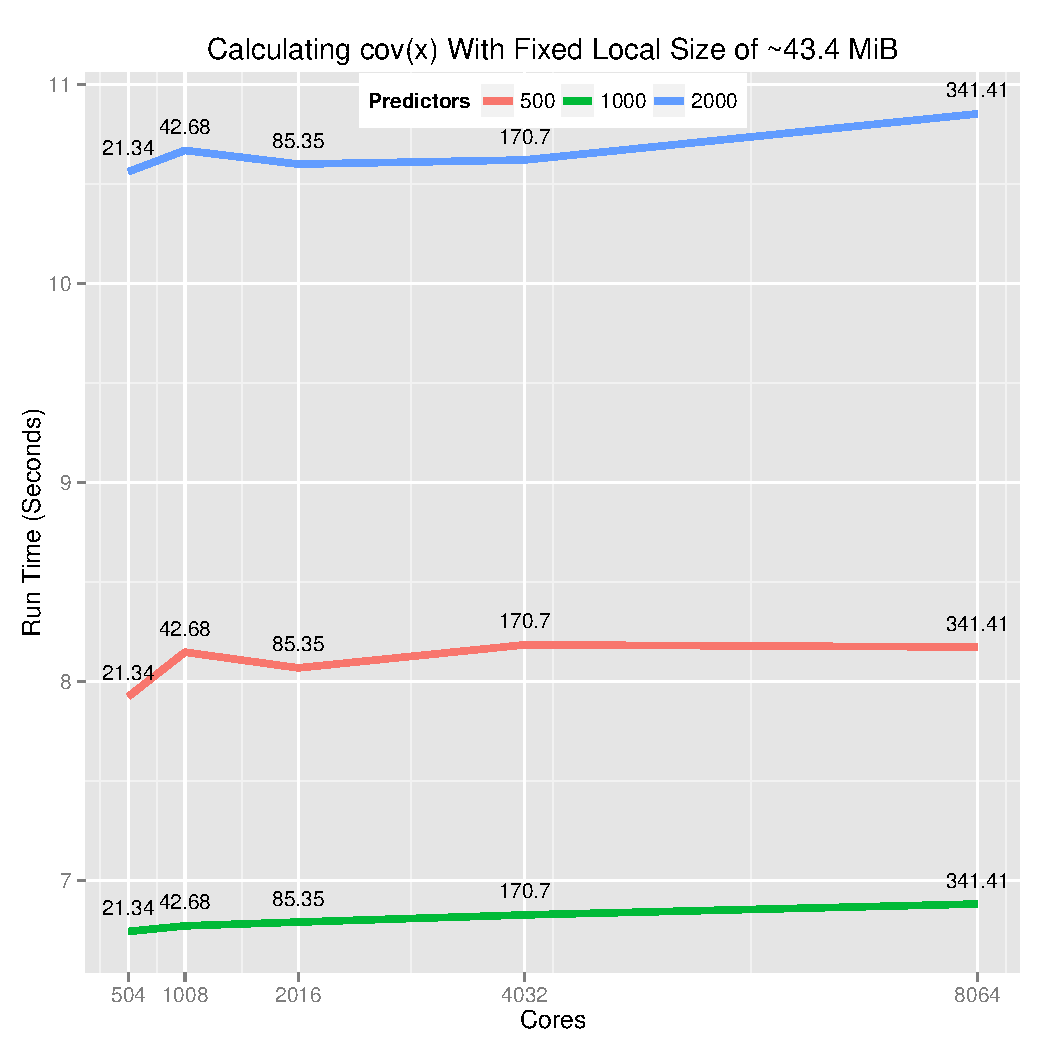
\includegraphics[height=.88\textheight]{../common/pics/cov}
  \end{center}
  \end{block}
\end{frame}



% \subsection{Linear Model Fitting}

\begin{frame}[fragile]
  \begin{block}{Linear Model Code}
\begin{lstlisting}
x <- ddmatrix("rnorm", nrow=n, ncol=p, mean=mean, sd=sd)
beta_true <- ddmatrix("runif", nrow=p, ncol=1)

y <- x %*% beta_true

beta_est <- lm.fit(x=x, y=y)$coefficients 
\end{lstlisting}
  \end{block}
\end{frame}

\begin{frame}
  \begin{block}{\code{Data Generation}}
  \begin{center}
    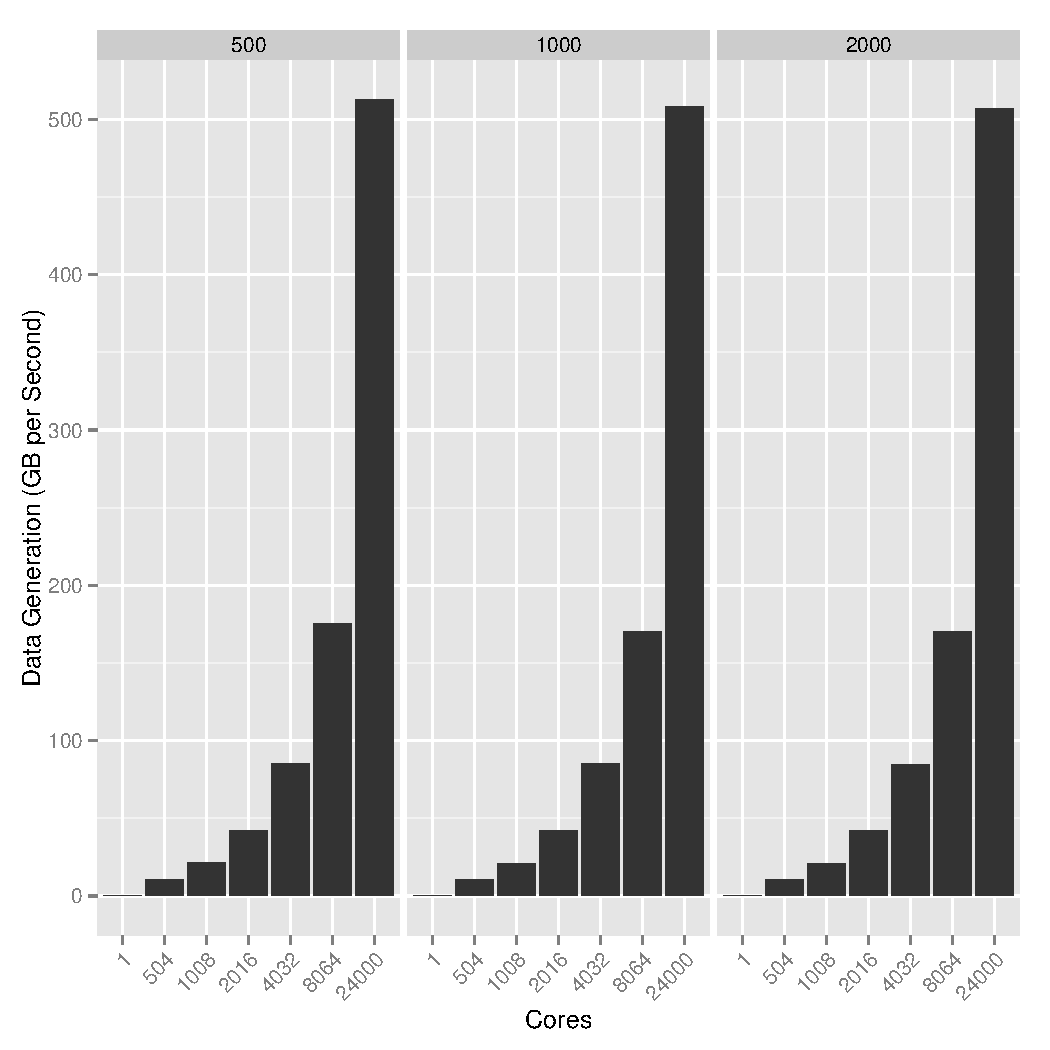
\includegraphics[height=.88\textheight]{../common/pics/datagen}
  \end{center}
  \end{block}
\end{frame}

% \begin{frame}
%   \begin{block}{\code{lm.fit()}}
%   \begin{center}
%     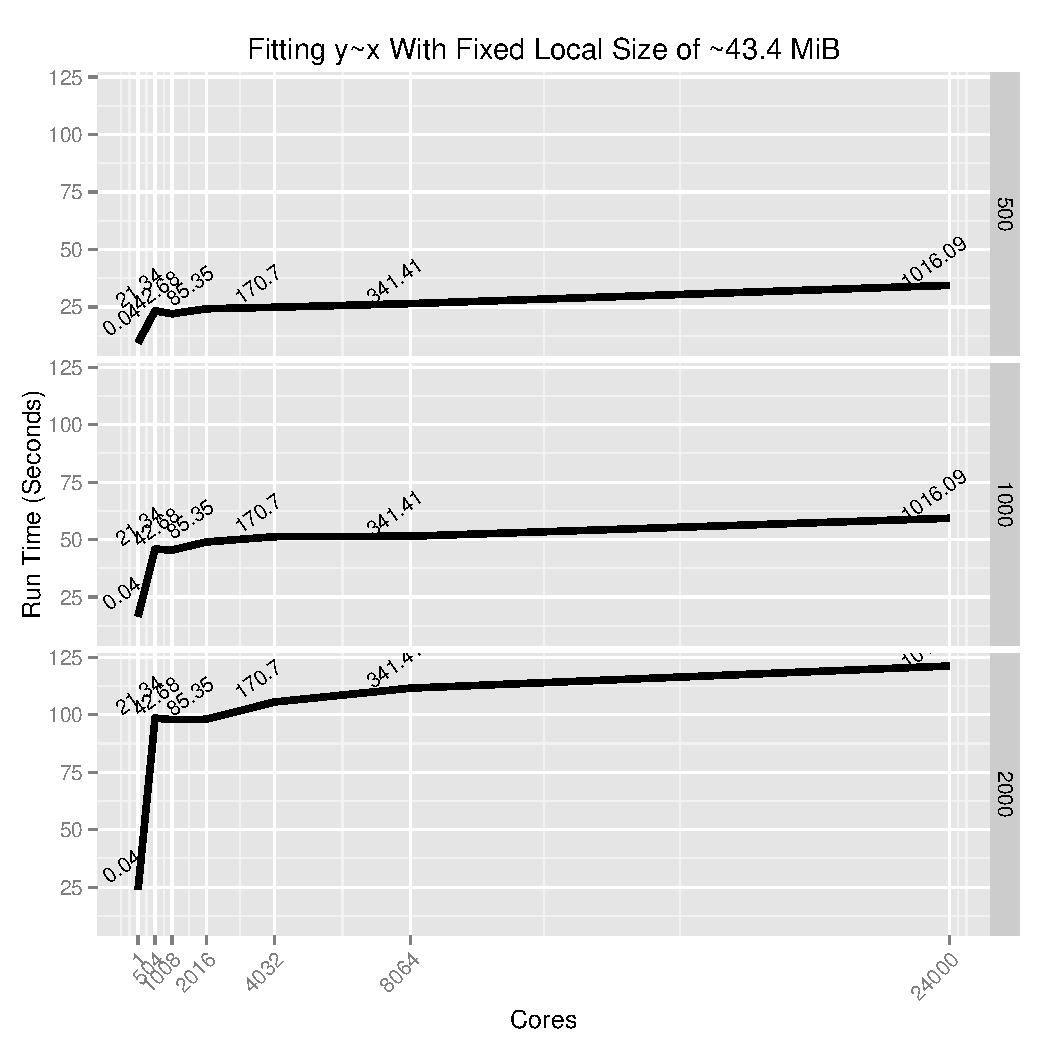
\includegraphics[height=.88\textheight]{../common/pics/lmfit1}
%   \end{center}
%   \end{block}
% \end{frame}

\begin{frame}
  \begin{block}{\code{lm.fit()}}
  \begin{center}
    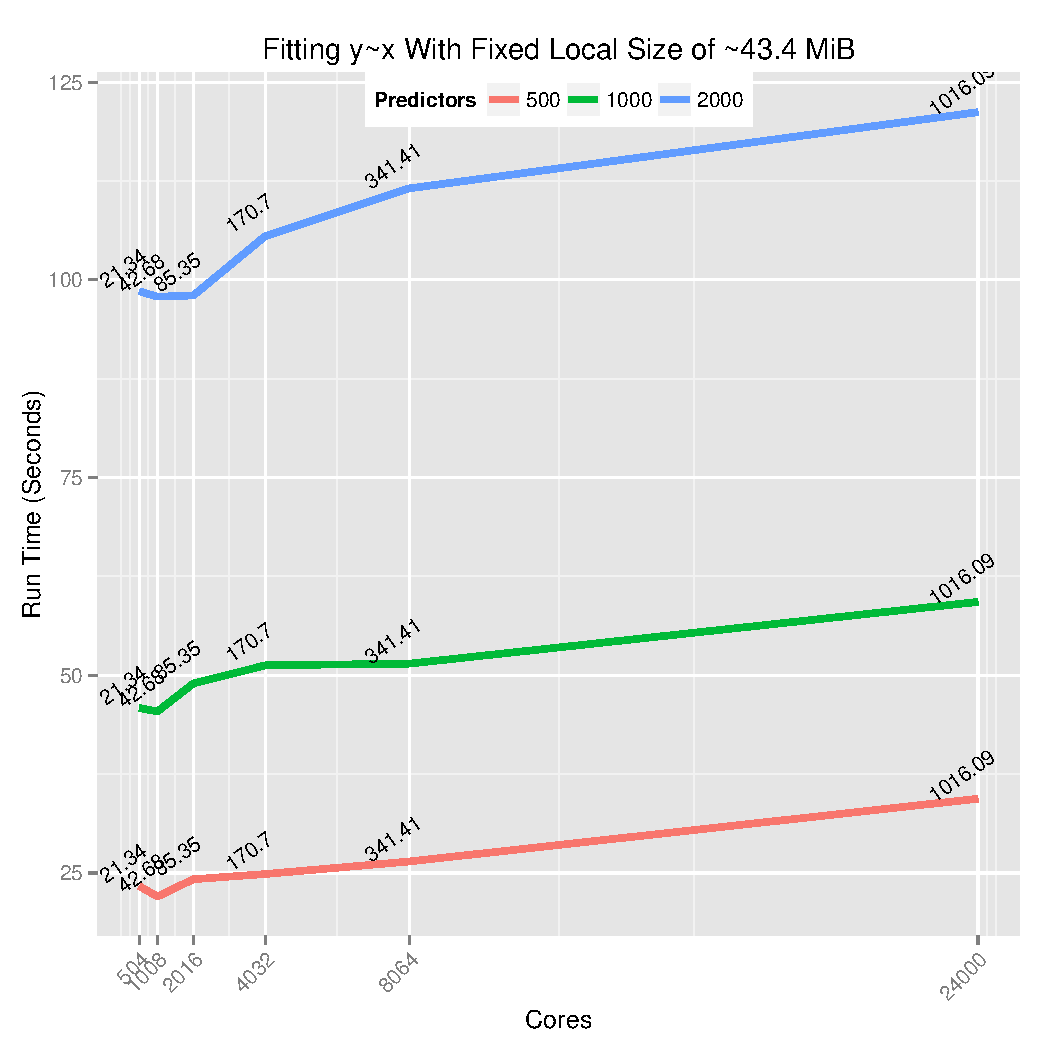
\includegraphics[height=.88\textheight]{../common/pics/lmfit2}
  \end{center}
  \end{block}
\end{frame}
\section{Challenges}

\hidenum
\begin{frame}[noframenumbering]
\frametitle{Contents}
 \tableofcontents[currentsection,hideallsubsections]
\end{frame}
\shownum


\subsection{Challenges}

\begin{frame}
  \begin{block}{Challenges}
    \begin{itemize}[<+-|alert@+>]
      \item Perceptions.
      \item Library loading.
      \item Profiling.
    \end{itemize}
  \end{block}
\end{frame}


\begin{frame}
  \begin{block}{Covariance Revisited: Distributed Data Parameter Calibration}
    \begin{center}
     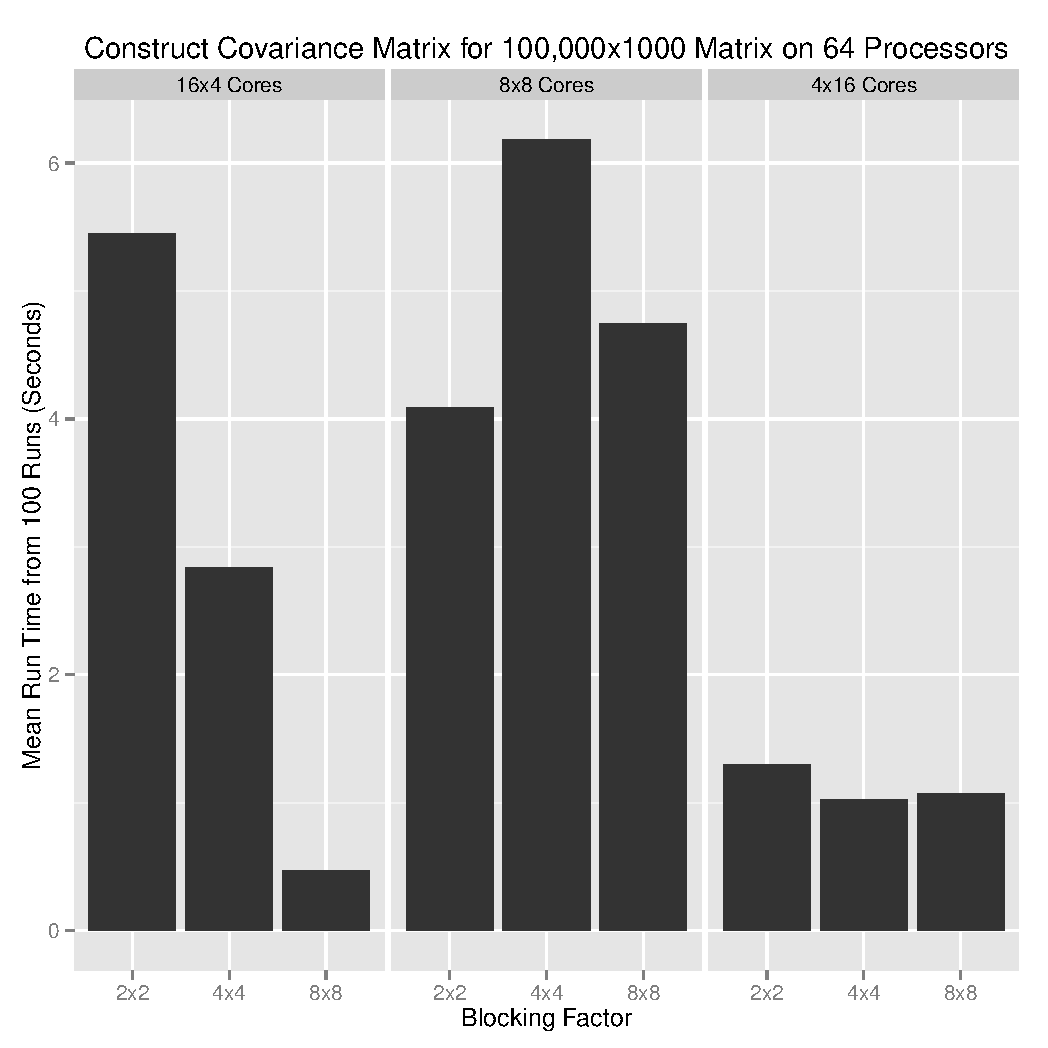
\includegraphics[width=10cm, height=7cm]{../common/pics/cov_param}
    \end{center}
  \end{block}
\end{frame}

\begin{frame}
  \begin{block}{Adding More Levels of Parallelism}
    \begin{center}
      {\color{dkblue}Distributed Memory (cluster nodes)} \\
      {\color{dkgreen}Shared Memory (multicore)} \\
      {\color{purple}Co-Processor (GPU, manycore)}
    \end{center}
    \begin{itemize}
      \item {\color{dkblue}pbdDMAT} + {\color{purple}CUBLAS}: near term on Titan 
      \item {\color{dkblue}pbdDMAT} - {\color{dkblue}ScaLAPACK} +
        {\color{dkblue}D}{\color{dkgreen}PLASMA}: QR only 
      \item {\color{dkblue}pbdDMAT} + {\color{dkgreen}PLASMA} or
        {\color{dkgreen}MKL} or {\color{dkgreen}ACML}: often helps 
      \item {\color{dkblue}pbdDMAT} + {\color{purple}MAGMA}: may not help 
    \end{itemize}
  \end{block}
\end{frame}

\hidenum
\section*{}
\begin{frame}[noframenumbering]
  \begin{block}{Tutorials}
  \begin{itemize}
    \item {\small OLCF Very Large Data Workshop
         ... {\color{red} NEXT!}}
    \item {\small Seoul National University, August 20}
    \item {\small SC13, November 17-22, Denver}
  \end{itemize}
  \end{block}
  \begin{block}{Invited Talks}
  \begin{itemize}
    \item {\small International Association for Statistical Computing, Aug 22-23, Seoul}
    \item {\small 59th ISI World Statistics Congress, August 25-30, Hong Kong }
  \end{itemize}
  \end{block}
\end{frame}
  
\begin{frame}[noframenumbering]
 \begin{block}{Thanks for coming!}
 \begin{center}
     {\Large Questions?}\\[1cm]
     {\Large Be sure to stick around for the tutorial!}
  \end{center}
 \end{block}
\end{frame}


\end{document}